\documentclass{thomasClass}

%\usepackage[firstpage]{draftwatermark}
%\SetWatermarkText{\textsc{proof}}
%\SetWatermarkScale{7}

\usepackage{appendix}

%----DEFINE PARAMETERS FOR THE LISTINGS PACKAGE----
\usepackage{listings}
\usepackage{amsmath}

\definecolor{codegreen}{RGB}{87,166,74}
\definecolor{codegray}{rgb}{0.5,0.5,0.5}
\definecolor{codepurple}{RGB}{214,157,133}
\definecolor{codeblue}{RGB}{86,156,214}
\definecolor{codenormal}{RGB}{220,220,220}

\lstdefinestyle{assembly}{
    backgroundcolor=\color{white},   
    commentstyle=\color{codegreen},
    keywordstyle=\color{codeblue},
    numberstyle=\tiny\color{codegray},
    stringstyle=\color{codepurple},
    basicstyle=\ttfamily\small\color{black},
    breakatwhitespace=false,         
    breaklines=true,                 
    captionpos=b,                    
    keepspaces=true,                 
    numbers=left,                    
    numbersep=5pt,                  
    showspaces=false,    
    showstringspaces=false,
    showtabs=false,                  
    tabsize=2,
    rulecolor=\color{black},
    postbreak=\mbox{\textcolor{red}{$\hookrightarrow$}\space},
    morekeywords={goto, return, btfss, btfsc, bcf, movlw, movf, decfsz},
}

%MAKE PAGE HEADERS
\usepackage{fancyhdr}
\pagestyle{fancy}
\fancyhf{}
\fancyhead[LE,RO]{Thomas Boxall}
\fancyhead[RE,LO]{A-Level Electronics - Task 1} %put project title here
\fancyfoot[RE,LO]{}
\fancyfoot[LE,RO]{\thepage}
\renewcommand{\footrulewidth}{0.4pt}
\addtolength{\topmargin}{-1.59999pt}
\setlength{\headheight}{13.59999pt}


\begin{document}
\begin{titlepage} % Suppresses headers and footers on the title page
	
	\centering % Centre everything on the title page
	
	%------------------------------------------------
	%	Top rules
	%------------------------------------------------
	
	\rule{\textwidth}{1pt} % Thick horizontal rule
	
	\vspace{2pt}\vspace{-\baselineskip} % Whitespace between rules
	
	\rule{\textwidth}{0.4pt} % Thin horizontal rule
	
	\vspace{0.1\textheight} % Whitespace between the top rules and title
	
	%------------------------------------------------
	%	Title
	%------------------------------------------------

	{\Huge \textbf{A-Level Electronics Project}}\\[0.5\baselineskip] % Title line 1
	{\huge Task 2 - Electronic System}\\[0.5\baselineskip] % Title line 2
	{\LARGE Voltmeter} % Title line 3

	
	\vspace{0.025\textheight} % Whitespace between the title and short horizontal rule
	
%	\rule{0.3\textwidth}{0.4pt} % Short horizontal rule under the title
% make a voltmeter symbol in place of short horizontal rule under the title
\begin{circuitikz}
    \centering
    \draw
    (0,0) to[rmeter, t=V] (4,0);
\end{circuitikz}
	
	\vspace{0.1\textheight} % Whitespace between the thin horizontal rule and the author name
	
	%------------------------------------------------
	%	Author
	%------------------------------------------------
	
	{\Large \textsc{Thomas Boxall}} \\% Author name
	{\large\textsc{march 2022}} % Date
	
	\vfill % Whitespace between the author name and publisher
	
	%------------------------------------------------
	%	Extra info
	%------------------------------------------------
	
	{\large\textsc{BEXHILL COLLEGE: 56635}} \\
	{\large\textsc{CANDIDATE NO: 5377}}
	
	\vspace{0.1\textheight} % Whitespace under the date text
	
	%------------------------------------------------
	%	Bottom rules
	%------------------------------------------------
	
	\rule{\textwidth}{0.4pt} % Thin horizontal rule
	
	\vspace{2pt}\vspace{-\baselineskip} % Whitespace between rules
	
	\rule{\textwidth}{1pt} % Thick horizontal rule
	
\end{titlepage}

\ \\ \newpage
\tableofcontents
\newpage

\chapter{Introduction}

\section{Introduction to the Project}
Traffic lights are fundamental to the smooth running of the road networks. Without them vehicle drivers would be placed in potentially dangerous situations multiple times per journey, where they approach junctions with multiple roads; not to mention the risk which pedestrians would take every time they cross the road. Traffic lights (amongst other electronically controlled traffic management systems) provide some order to what would otherwise be uncontrolled chaos.\newline
I chose those this project with the aim of understanding how a traffic light control system works as well as understanding how microcontrollers work, interfacing with their inputs and outputs. Whilst the unknown of how microcontrollers work added to the complexity, the comfort of using traffic lights daily makes this feel like its a manageable task to complete in the time allocated. 

\section{Definition of Traffic Lights}
Everyone knows what traffic lights do, but for this project I feel it is deeply important to have an understanding of the definition of a traffic lights. \newline
Collins English Dictionary\footnote{https://www.collinsdictionary.com/dictionary/english/traffic-light} defines 'Traffic Lights' as:
\blockQuote{Traffic lights are sets of red, amber, and green lights at the places where roads meet. They control the traffic by signalling when vehicles have to stop and when they can go. Traffic lights can also be referred to as a traffic light.}
\chapter{Research}
Before I start to design my traffic light control system, I need to research existing designs, to understand both how they work and how they are controlled.

\section{How Traffic Lights Work}
Traffic lights are generally divided into two categories, they will either be based off of a timing circuit or they will have some form of vehicle sensor which will trigger the changing of the lights. Each of these have their own pros and cons. Sometimes a combination of the two is preferred.

\subsection{Systems with Vehicle Sensors}
Traffic light control systems which are based off of a vehicle sensor or sensors alone are generally inadequate for for junctions in areas with a higher population density. Using the diagram below (fig. \ref{fig:bridgeDiagram} as an example; the blue cars are able to cross the bridge, but as there are blue cars constantly arriving at traffic light set A, the system doesn't see that there are cars waiting at traffic light set B therefore it doesn't change. This means that there is a pile up of cars at traffic lights B.
\begin{figure}[H]
    \centering
    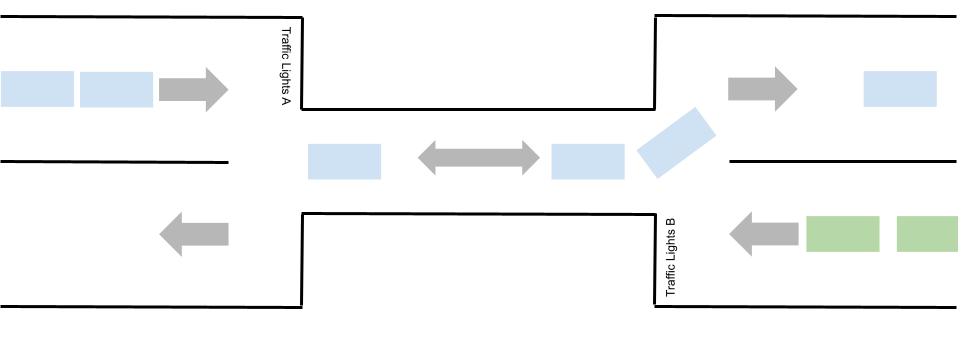
\includegraphics[width=0.8\textwidth]{images/Bridge diagram.png}
    \caption{Diagram of traffic flow over a bridge}
    \label{fig:bridgeDiagram}
\end{figure}

\subsection{Systems with Timers}
Traffic light control systems which are based off of a timer alone are generally more suited for areas which receive higher levels of traffic. This is because they allow one set of traffic to move for a set length of time then allow the other set to move for a set length of time, then repeats.

\subsection{Systems with Timers and Vehicle Sensors}
Traffic light control systems which are based off of a timer and vehicle sensor(s) are the most efficient, however with the added efficiency comes additional complexity. This is the best type of system as (using the diagram in Fig. \ref{fig:bridgeDiagram}) the system would be able to tell that the blue cars have had a chance to go and there are green cars waiting therefore it can let the green cars go.


\section{Traffic Light Controlled Junctions}
There are a number of different types of traffic light and pedestrian crossing systems\footnote{https://www.highwaycodeuk.co.uk/rules-for-pedestrians-crossings.html}, each has a different priority pattern and each uses a different combination of vehicle/pedestrian sensors and timing systems.

\subsection{EXAMPLE 1: Two-Way Traffic Lights}
\begin{figure}[H]
    \centering
    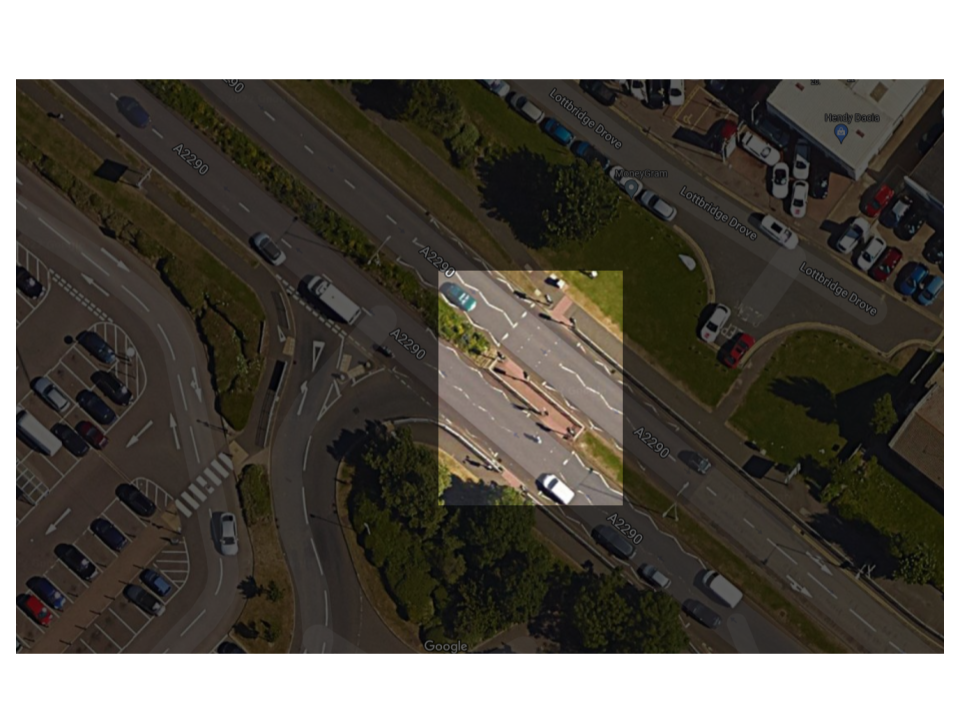
\includegraphics[width=0.8\textwidth]{images/Simple TL junction outside tesco.png}
    \caption{Image of the two-way junction}
    \label{fig:tesoTrafficLights}
\end{figure}
\noindent \textit{Data from Google Maps (2022). Available from:\\ https://www.google.com/maps/@50.7865833,0.3056209,74m/data=!3m1!1e3 [Accessed 13 03 2022]}\newline

\noindent This junction has two identical sections to it. Each has a set of traffic lights to stop a single carriageway of traffic and a pedestrian crossing to allow pedestrians to cross the dual carriage which this is situated on. Due to the fact that this is on a dual carriageway, it can safely be assumed that this traffic light system is controlled by the pedestrian crossing alone, without any vehicle sensors or timing control systems. This assumption would work by the pedestrian pressing the button which indicates to the system that they are ready to cross then the system waiting a set length of time, allow the pedestrians to cross for a set length of time then return to a green light for the traffic.

\subsection{EXAMPLE 2: Complex Junction}
\begin{figure}[H]
    \centering
    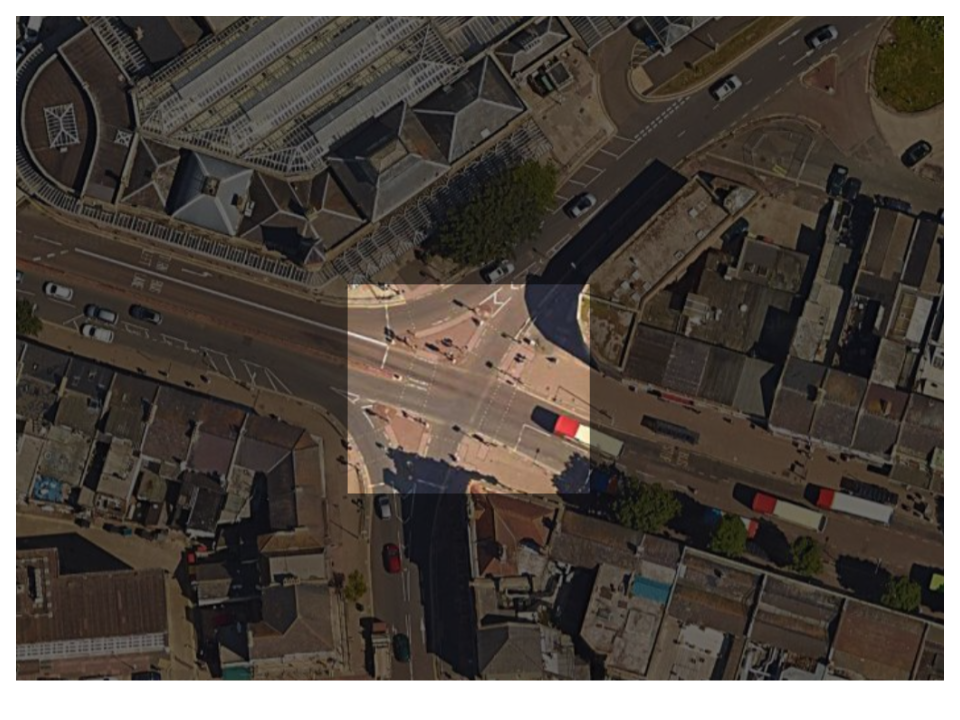
\includegraphics[width=0.8\textwidth]{images/Complex junction.png}
    \caption{Image of the complex junction}
    \label{fig:complexJunction}
\end{figure}
\noindent \textit{Data from Google Maps (2022). Available from:\\ https://www.google.com/maps/@50.7690679,0.2817194,121m/data=!3m1!1e3 [Accessed 13 03 2022]}\newline

\noindent This is a much more complicated junction where there are multiple lanes of traffic which converge into single lanes as well as pedestrians which have to cross. I assume this is controlled using a mixture of timings and pedestrian triggers. The big difference between this junction and the junction above is that this junction can allow pedestrians to cross simultaneously while vehicles also move, making it more efficient.
\chapter{Design}

\section{Specification}
\begin{enumerate}
    \item The traffic light control system should be easy to use.
    \item The traffic light control system should be as efficient as possible, reducing heat dissipated to the environment.
    \item The traffic light control system should recieve an input from a pedestrian and take 40 seconds ($\pm$20s) to allow them to cross.
    \item The traffic light control system should not favour any particular road user over an other as well as giving equal chances to all direction of traffic.
    \item The traffic light system should ensure that when a direction of traffic is not able to go, its red stop LED is illuminated.
    \item The traffic light control system should take a 0V and +5V (within $\pm$0.5V) input.
    \item The traffic light control system should alert 'pedestrians' in at least two different ways that it is their turn to cross.
    \item The traffic light control system should be developed in a way such that, the code is clear to read and understand, to ensure future developments can be carried out easily.
\end{enumerate}

\section{Junction design}
Now I have my specification, I am able to design the junction which I will design the traffic light control system for. I will be using a junction in my home town (Eastbourne) as inspiration.
\subsection{Real Life Junction}
\begin{figure}[H]
    \centering
    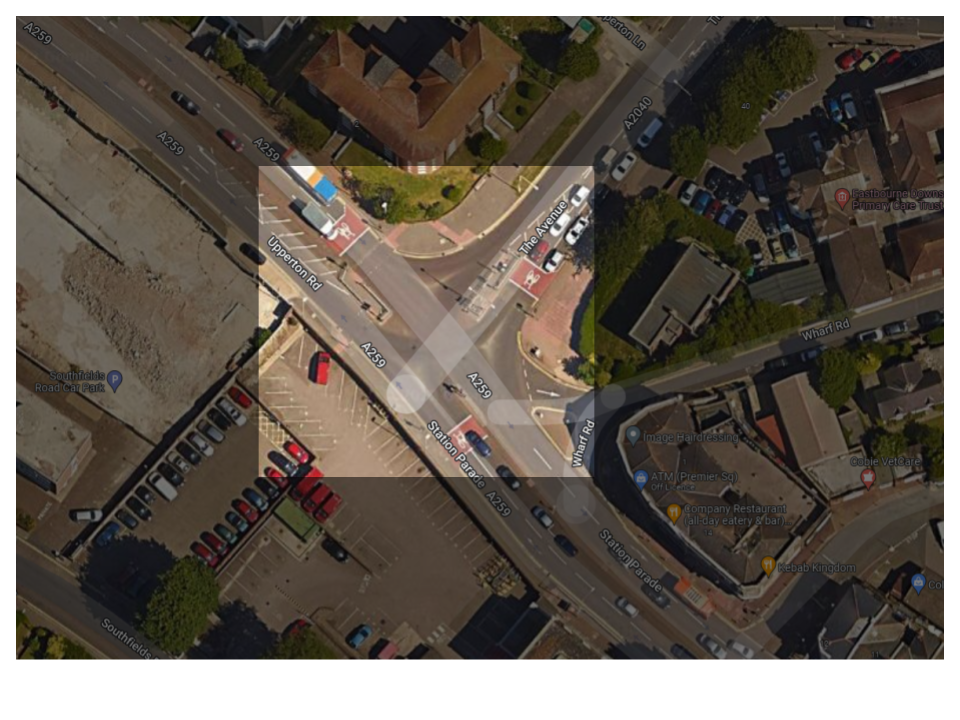
\includegraphics[width=0.9\textwidth]{images/IRL diagram.png}
    \caption{Image of the inspiration junction}
    \label{fig:IRLJunction}
\end{figure}
\noindent \textit{Data from Google Maps (2022). Available from:\\ https://www.google.com/maps/@50.7701274,0.2786944,118m/data=!3m1!1e3 [Accessed 13 03 2022]}\newline

\noindent This is a three-way traffic light controlled junction with pedestrian crossing for two of the three ways. 

\subsection{Abstracted Junction}
\begin{figure}[H]
    \centering
    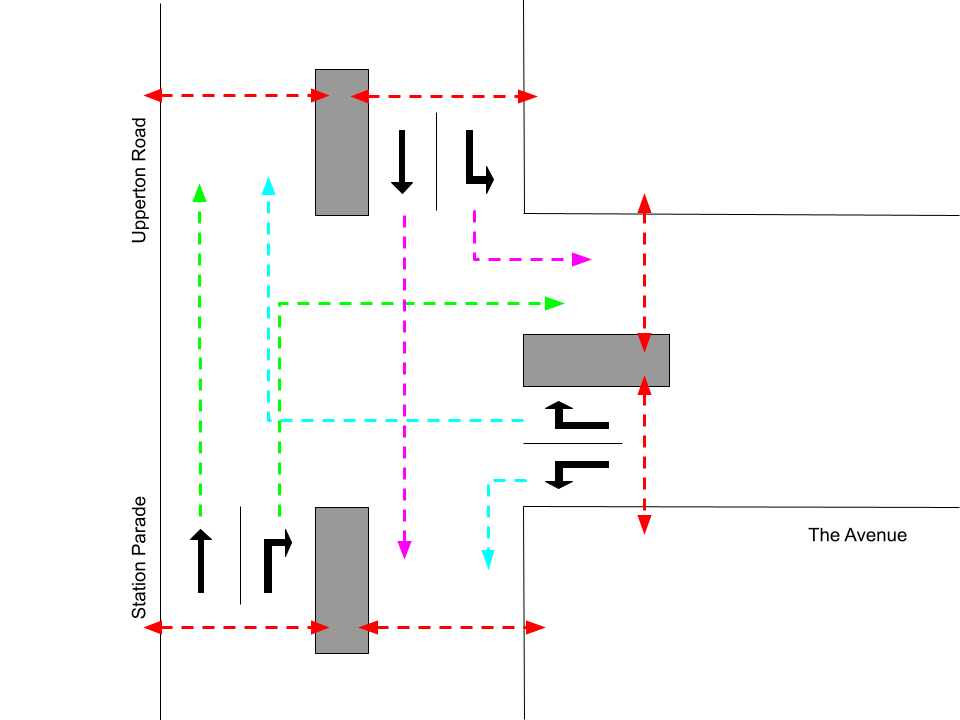
\includegraphics[width=0.8\textwidth]{images/Abstracted diagram.png}
    \caption{Diagram of the junction used in this project}
    \label{fig:abstractedDiagram}
\end{figure}
\noindent The diagram above shows an abstracted version of the junction shows in figure \ref{fig:IRLJunction}. This abstracted version has four colours dashed lines drawn on it. These show the routes which can be taken by either the pedestrians or cars. The red route indicates a pedestrian crossing. The blue, pink and green lines indicate routes which can be taken by vehicles. The grey boxes indicate pedestrian islands. Additional pedestrian crossing routes have been included in my abstracted diagram. This is because in the real junction, the areas which do not have pedestrian crossings are extremely dangerous as cars travel at high speeds.

\section{Traffic Light Sequence}
After working out the type of junction I will design an traffic light control system for, I am now able to work out the sequence which the traffic lights will cycle through. At this point, I have also decided that the traffic light sequence will be contained within a subroutine; hence the references about 'Main Program' in the diagram below.
\begin{figure}[H]
    \centering
    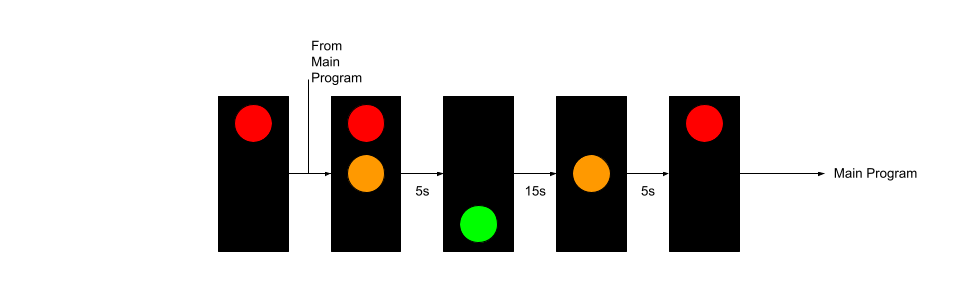
\includegraphics[width=0.9\textwidth]{images/Traffic light sequence.png}
    \caption{Sequence of lights in the traffic lights}
    \label{fig:trafficLightSequence}
\end{figure}

\section{Inputs and Outputs}
The PIC16F88 microcontroller has 16 input output bits, divided into two 'ports' of 8 (PORTA and PORTB).
In my system, all inputs and outputs will be active high (logic 1).
\begin{figure}[H]
    \begin{minipage} {0.45\textwidth}
        \subsection{PORTA}
        \begin{itemize}
            \item[0] Output, red LED
            \item[1] Output, amber LED
            \item[2] Output, green LED
            \item[3] Output, red LED
            \item[4] Output, amber LED
            \item[5] 
            \item[6] Output, red LED
            \item[7] Output, amber LED
        \end{itemize}
    \end{minipage}\hfill
    \begin{minipage} {0.45\textwidth}
        \subsection{PORTB}
        \begin{itemize}
            \item[0] Output, green LED
            \item[1] Input, button
            \item[2] Output, white LED
            \item[3] Output, red LED
            \item[4] Output, green LED
            \item[5] Output, buzzer
            \item[6] 
            \item[7] Output, green LED
        \end{itemize}
    \end{minipage}
\end{figure}


\section{Component of the control system}
The control system will be based off of a PIC16F88 microcontroller, this will be the heart of the system. Alongside the microcontroller, I will also need some LEDs (in red, amber and green), a buzzer and a button.
\subsection{Components list}
\begin{itemize}
    \item 4 red LEDs
    \item 4 green LEDs
    \item 3 amber LEDs
    \item 1 white LED
    \item 2 eight 220K$\Omega$ resistor packs
    \item 3 220k$\Omega$ resistors
    \item 1 1K$\Omega$ resistor
    \item 1 Push-To-Make button
    \item 1 PIC16F88 Microcontroller
\end{itemize}
In reality, my circuit will only need 12 220K$\Omega$ resistors. However, for convenience, and minimising the number of components on the breadboards, it is easier to use 2 resistor packs and a number of loose resistors.



\chapter {Algorithm Design}

%have each subroutine listed with subroutine name as section then subsecs for flowchart, intital code, debugging and testing etc.
After planning my traffic light control system, I can now begin to design the algorithms. Looking at the exam board template provided to us, it is clear that the microcontroller can run subroutines as well as a procedural main program code section. \newline
Using subroutines is the most efficient way to program as it allows you to use the same lines of code a number of times, not only does this reduce the total number of lines of code you have to program but it also reduces the number of lines of code which are flashed onto the microcontroller. Using this knowledge, I designed my main program to call a number of subroutines. \newline

\noindent \textit{Shown below are the flowcharts and initial iteration of the algorithms. Full code listings are available in Appendix \ref{app:full-code}. Testing and debugging of the code is available in Chapter \ref{chap:testing}.}


\section{Main Program}
This code gets run automatically once the microcontroller has initialised. \newline
\noindent This algorithm works by initialising the stop LEDs by turning them all on. It then sequentially cycles through all of the sets of traffic lights, allowing them to cycle each time. After each set of traffic lights, it runs the \verb|checkPedstrian| algorithm which will check if there are pedestrians waiting to cross. This cycle repeats until the system is powered down.
\subsection*{Flowchart}
\begin{figure}[H]
    \centering
    
\includegraphics[width=0.9\textwidth]{images/flowchart-main.png}
    \caption{Main program flowchart}
    \label{fig:flowchart-main}
\end{figure}
\subsection*{Code}
\begin{lstlisting}[language={[x86masm]Assembler}, style=assembly, caption=Main sequence code]
;first turn on all stop leds
	bsf PORTA, 0 ;turn on pink set stop eld
	bsf PORTA, 3 ;turn on green set stop led
	bsf PORTA, 6 ;turn on blue set stop led
	bsf PORTB, 3 ;turn on pedestrian stop led

mtop call pinkTrafficLightSequence
	call checkPedestrian
	call greenTrafficLightSequence
	call checkPedestrian
	call blueTrafficLightSequence
	call checkPedestrian
	goto mTop
\end{lstlisting}

\section{checkButton Subroutine}
This algorithm is used to check if the pedestrian button has been pressed and if it has, turn on the red wait LED which would be found at traffic lights with pedestrian crossings.

\subsection*{Flowchart}
\begin{figure}[H]
    \centering
    
\includegraphics[width=0.9\textwidth]{images/flowchart-checkButton.png}
    \caption{Check button subroutine flowchart}
    \label{fig:flowchart-checkButton}
\end{figure}
\subsection*{Code}
\begin{lstlisting}[language={[x86masm]Assembler}, style=assembly, caption=checkButton subroutine]
;function to check the button
checkButton
	btfss PORTB, 1 ;skip next line of code if button pressed (active high)
	return ;can go back to where called from
	bsf PORTB, 2 ;turn red wait LED on
	return ;go back to main code
;end of function
\end{lstlisting}

\section{checkPedestrian Subroutine}
This algorithms is used to read the current state of the pedestrian wait LED. Depending on this state, it will either return straight to the main code or run the \verb|cyclePedestrian| subroutine.

\subsection*{Flowchart}
\begin{figure}[H]
    \centering
    
\includegraphics[width=0.9\textwidth]{images/flowchart-checkPedestrian.png}
    \caption{checkPedestrain subroutine flowchart}
    \label{fig:flowchart-chechPedestrian}
\end{figure}
\subsection*{Code}
\begin{lstlisting}[language={[x86masm]Assembler}, style=assembly, caption=checkPedestrian subroutine]
checkPedestrian
	;function to check if the wait led is on
		;if yes - cycle pedestrian crossing
		;if no - return to main 
	btfsc PORTB, 2 ;skip next line if wait led NOT on therefore if on, run next line
	call cycleCrossing
	return
;end function
\end{lstlisting}

\section{cycleCrossing Subroutine}
This algorithm will control the pedestrian crossing to allow the pedestrians to cross. 
\subsection*{Flowchart}
\begin{figure}[H]
    \centering
    
\includegraphics[width=0.9\textwidth]{images/flowchart-pedCrossingCycle.png}
    \caption{cycleCrossing subroutine flowchart}
    \label{fig:flowchart-cyclePedCrossing}
\end{figure}
\subsection*{Code}
\begin{lstlisting}[language={[x86masm]Assembler}, style=assembly, caption=cycleCrossing subroutine]
; function to cycle the pedestrian crossing
cycleCrossing
	bcf PORTB, 2 ;turn off red wait LED
	bcf PORTB, 3 ;turn off red stop LED
	bsf PORTB, 4 ;turn on green go LED
	bsf PORTB, 5 ;turn on buzzer
	call wait1000ms ;wait 1second
	call wait1000ms ;wait 1second
	call wait1000ms ;wait 1second
	call wait1000ms ;wait 1second
	call wait1000ms ;wait 1second
	call wait1000ms ;wait 1second
	call wait1000ms ;wait 1second
	call wait1000ms ;wait 1second
	call wait1000ms ;wait 1second
	call wait1000ms ;wait 1second
	call wait1000ms ;wait 1second
	call wait1000ms ;wait 1second
	call wait1000ms ;wait 1second
	call wait1000ms ;wait 1second
	call wait1000ms ;wait 1second
	call wait1000ms ;wait 1second
	call wait1000ms ;wait 1second
	call wait1000ms ;wait 1second
	call wait1000ms ;wait 1second
	call wait1000ms ;wait 1second
	;now have waited 20seconds so invert things and return to main sequence
	bcf PORTB, 4 ;turn off green go LED
	bsf PORTB, 3 ;turn on red stop LED
	bcf PORTB, 5 ;turn off buzzer
	return ;return to the main program
;end of function
\end{lstlisting}

\section{wait5SecondsCheckButton Subroutine}
This algorithm is much more complicated that I originally anticipated it to be. What I wanted it to do was to wait 10ms then run the \verb|checkButton| subroutine. To do this, I would have a loop which counted to 500. This is not possible using this PIC microcontroller as it has a maximum number size of 256. To get around this, I am using two loops, X and Y. This will allow me to wait for five seconds and every 10ms of that, check if the button is pressed or not.
\subsection*{Flowchart}
\begin{figure}[H]
    \centering
    
\includegraphics[width=0.9\textwidth]{images/flowchart-wait5Sec.png}
    \caption{wait5SecondsCheckButton subroutine flowchart}
    \label{fig:flowchart-wait5Sec}
\end{figure}
\subsection*{Code}
\begin{lstlisting}[language={[x86masm]Assembler}, style=assembly, caption=wait5SecondsCheckButton subroutine]
waitFiveSecondsCheckButton
	;first, stary loop x
	movlw d'51' ;set val of 51 into w register
	movf loopX ; move the val in the working register (51) into loopX

topX decfsz loopX, 1 ;decrement loopX and place the new value back into loopX
	goto startY ;line skipped if result is 0
	return

startY movlw d'101'; ;set value of 101 into w register
	movf loopY ;move value in working register (101) into loopY

topY decfsz loopY, 1 ;decrement loopY and place new value back into loopY
	goto finalPart ;goto final part of the function
	goto startX ;run if loopY = 0

finalPart call checkButton
	call wait10ms ;wait for 10ms function
	goto startY ;go back up to startY and loop around again
;end of function
\end{lstlisting}

\section{Traffic lights}
The traffic light control algorithm is fundamentally the same for the three sets of traffic lights. This is shown in the flowchart, as there is only one for the three subroutines. The only difference between the three sets is which IO bits are changed.
\subsection*{Flowchart}
\begin{figure}[H]
    \centering
    
\includegraphics[width=0.9\textwidth]{images/flowchart-trafficLights.png}
    \caption{trafficLights subroutine flowchart}
    \label{fig:flowchart-trafficLights}
\end{figure}

\subsection*{Code}
\subsubsection*{Pink set}
\begin{lstlisting}[language={[x86masm]Assembler}, style=assembly, caption=Pink Traffic Light sequence]
pinkTrafficLightSequence
	bsf PORTA, 1 ;turn on amber led
	call waitFiveSecondsCheckButton ;wait 5s
	bcf PORTA, 1 ;turn off amber led
	bcf PORTA, 0 ;turn off red led
	bsf PORTA, 2 ; turn on greeen led
	call waitFiveSecondsCheckButton
	call waitFiveSecondsCheckButton
	call waitFiveSecondsCheckButton
	bcf PORTA, 2 ;turn off green led
	bsf PORTA, 1 ;turn on amber led
	call waitFiveSecondsCheckButton
	bsf PORTA, 0 ;turn on red led
	bcf PORTA, 1 ;turn off amber led
	return ;go back to main code
;end of function
\end{lstlisting}
\subsubsection*{Green set}
\begin{lstlisting}[language={[x86masm]Assembler}, style=assembly, caption=Green Traffic Light sequence]
greenTrafficLightSequence
	bsf PORTA, 4 ;turn on amber led
	call waitFiveSecondsCheckButton ;wait 5s
	bcf PORTA, 4 ;turn off amber led
	bcf PORTA, 3 ;turn off red led
	bsf PORTA, 5 ; turn on greeen led
	call waitFiveSecondsCheckButton
	call waitFiveSecondsCheckButton
	call waitFiveSecondsCheckButton
	bcf PORTA, 5 ;turn off green led
	bsf PORTA, 4 ;turn on amber led
	call waitFiveSecondsCheckButton
	bsf PORTA, 3 ;turn on red led
	bcf PORTA, 4 ;turn off amber led
	return ;go back to main code
;end of function
\end{lstlisting}

\subsubsection*{Blue set}
\begin{lstlisting}[language={[x86masm]Assembler}, style=assembly, caption=Blue Traffic Light sequence]
blueTrafficLightSequence
	bsf PORTA, 7 ;turn on amber led
	call waitFiveSecondsCheckButton ;wait 5s
	bcf PORTA, 7 ;turn off amber led
	bcf PORTA, 6 ;turn off red led
	bsf PORTB, 0 ; turn on greeen led
	call waitFiveSecondsCheckButton
	call waitFiveSecondsCheckButton
	call waitFiveSecondsCheckButton
	bcf PORTB, 0 ;turn off green led
	bsf PORTA, 7 ;turn on amber led
	call waitFiveSecondsCheckButton
	bsf PORTA, 6 ;turn on red led
	bcf PORTA, 7 ;turn off amber led
	return ;go back to main code
;end of function
\end{lstlisting}
\chapter{Testing}
\label{chap:testing}
Now I have designed the algorithms and developed the code. I can flash the microcontroller chip with the program. To do this, I will first need to compile the assembly language program into \verb|.hex| format which can be programmed onto it. \newline
\begin{figure}[H]
    \centering
    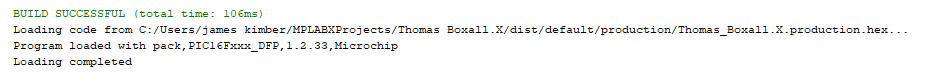
\includegraphics[width=0.9\textwidth]{images/compileSuccessful.png}
    \caption{Screenshot of MPLABX showing my code successfully compiling}
    \label{fig:compileSuccessful}
\end{figure}
\noindent After constructing the circuit as specified in my circuit design (\textit{Appendix \ref{chap:schematic})}, I connected the breadboard to power and let the program run \newline
This didn't work at first. After some troubleshooting, I realised that the problem was within the \verb|waitFiveSecondsCheckButton| subroutine. To fix this, I replaced it with a new subroutine, which only waited for one second, this mitigated the need for a second loop as I was only looping to 100, rather than 100 and 5 in two separate loops. This does increase the size of my program as I have to call the same function five times to achieve the same wait time as I would for the five second subroutine. This worked first time, and the microcontroller cycled through the traffic light sequence perfect first time. \newline
Now that the traffic lights are working, I am able to check if the pedestrian crossing is working and triggering correctly. To test this, I can press the button while the traffic lights are in a random state and observe the outcome. This worked first time, with the white wait LED turning on as soon as the button was pressed then when the current set of traffic lights reached the end of their sequence, the pedestrian crossing cycled as laid out in the design. The timings felt extremely out of proportion, so I reduced the crossing time to 3 seconds, this made the pedestrian crossing time feel better.
\begin{figure}[H]
    \centering
    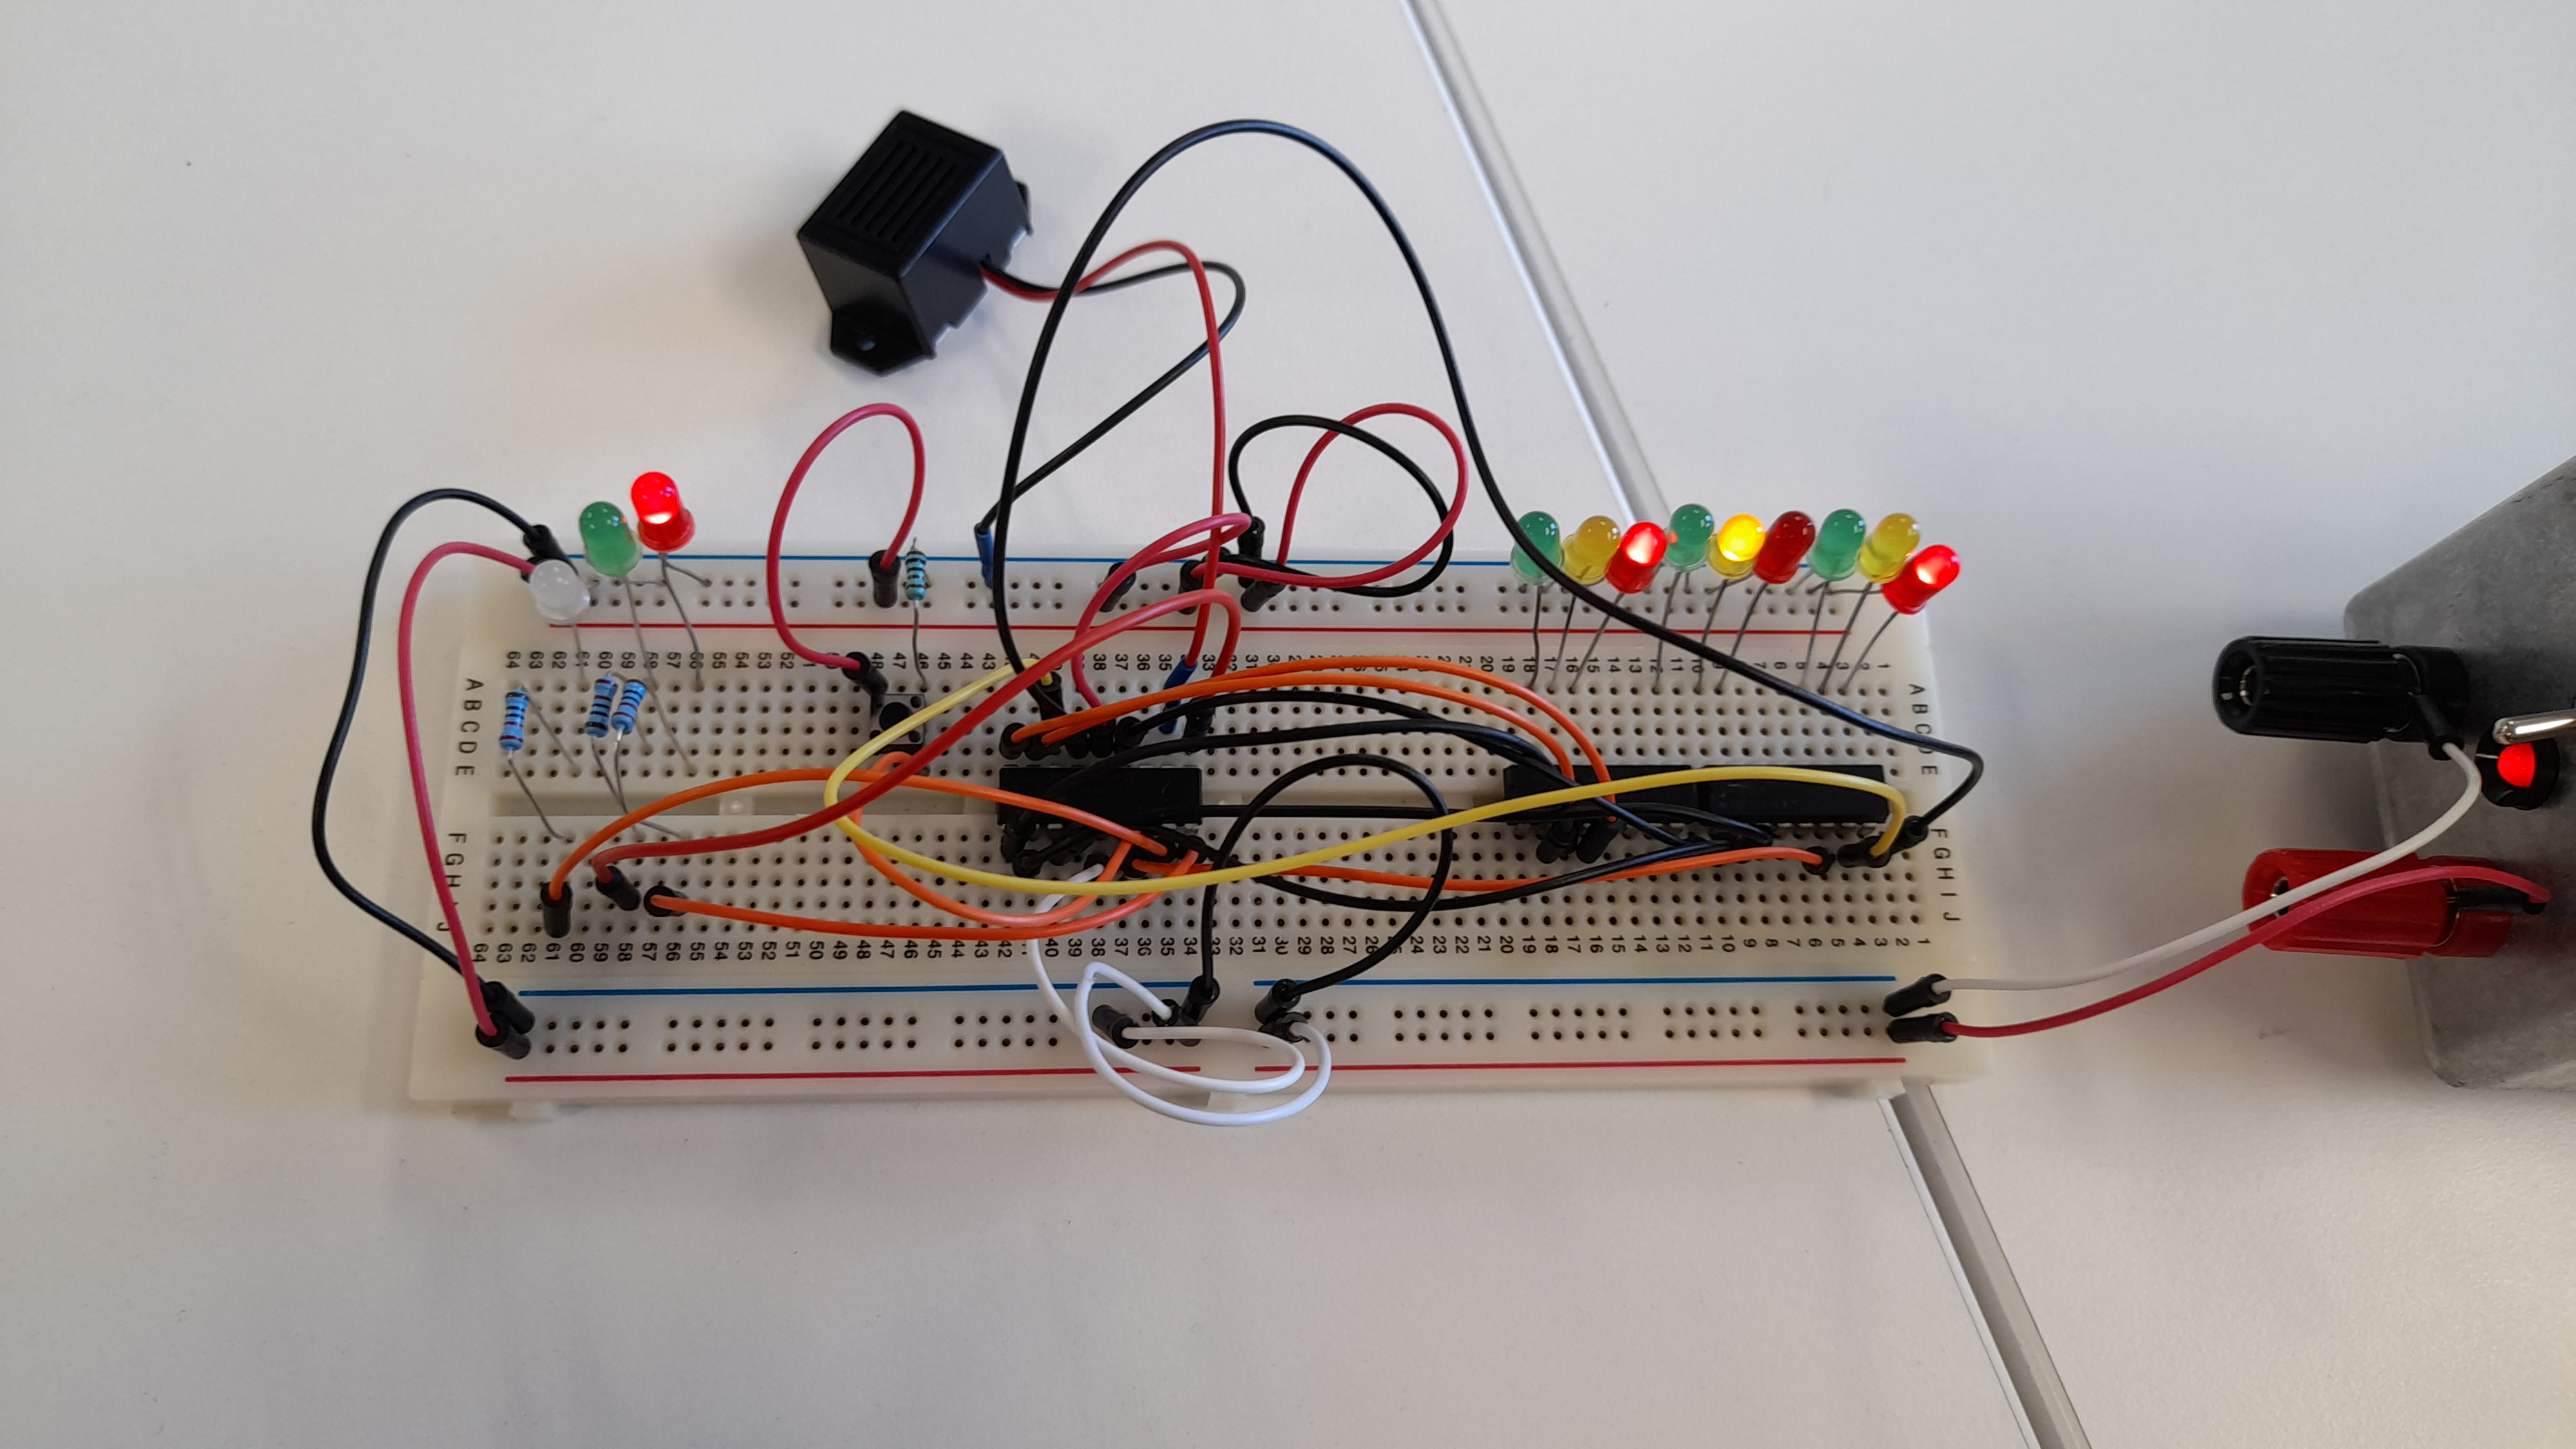
\includegraphics[width=0.9\textwidth]{images/unneatened.jpg}
    \caption{Circuit connected with temporary jumper wires}
    \label{fig:unneatened}
\end{figure}
\noindent This means that I have now completed construction of the system. I will now need to neaten the circuit.


\section{Sequence testing}
There are two different sets of sequences which I will need to check. One being the traffic light sequence and the other being the pedestrian crossing sequence.
\subsection{Traffic Lights sequence}
\begin{figure}[H]
    \begin{minipage}{0.45\textwidth}
        \centering
        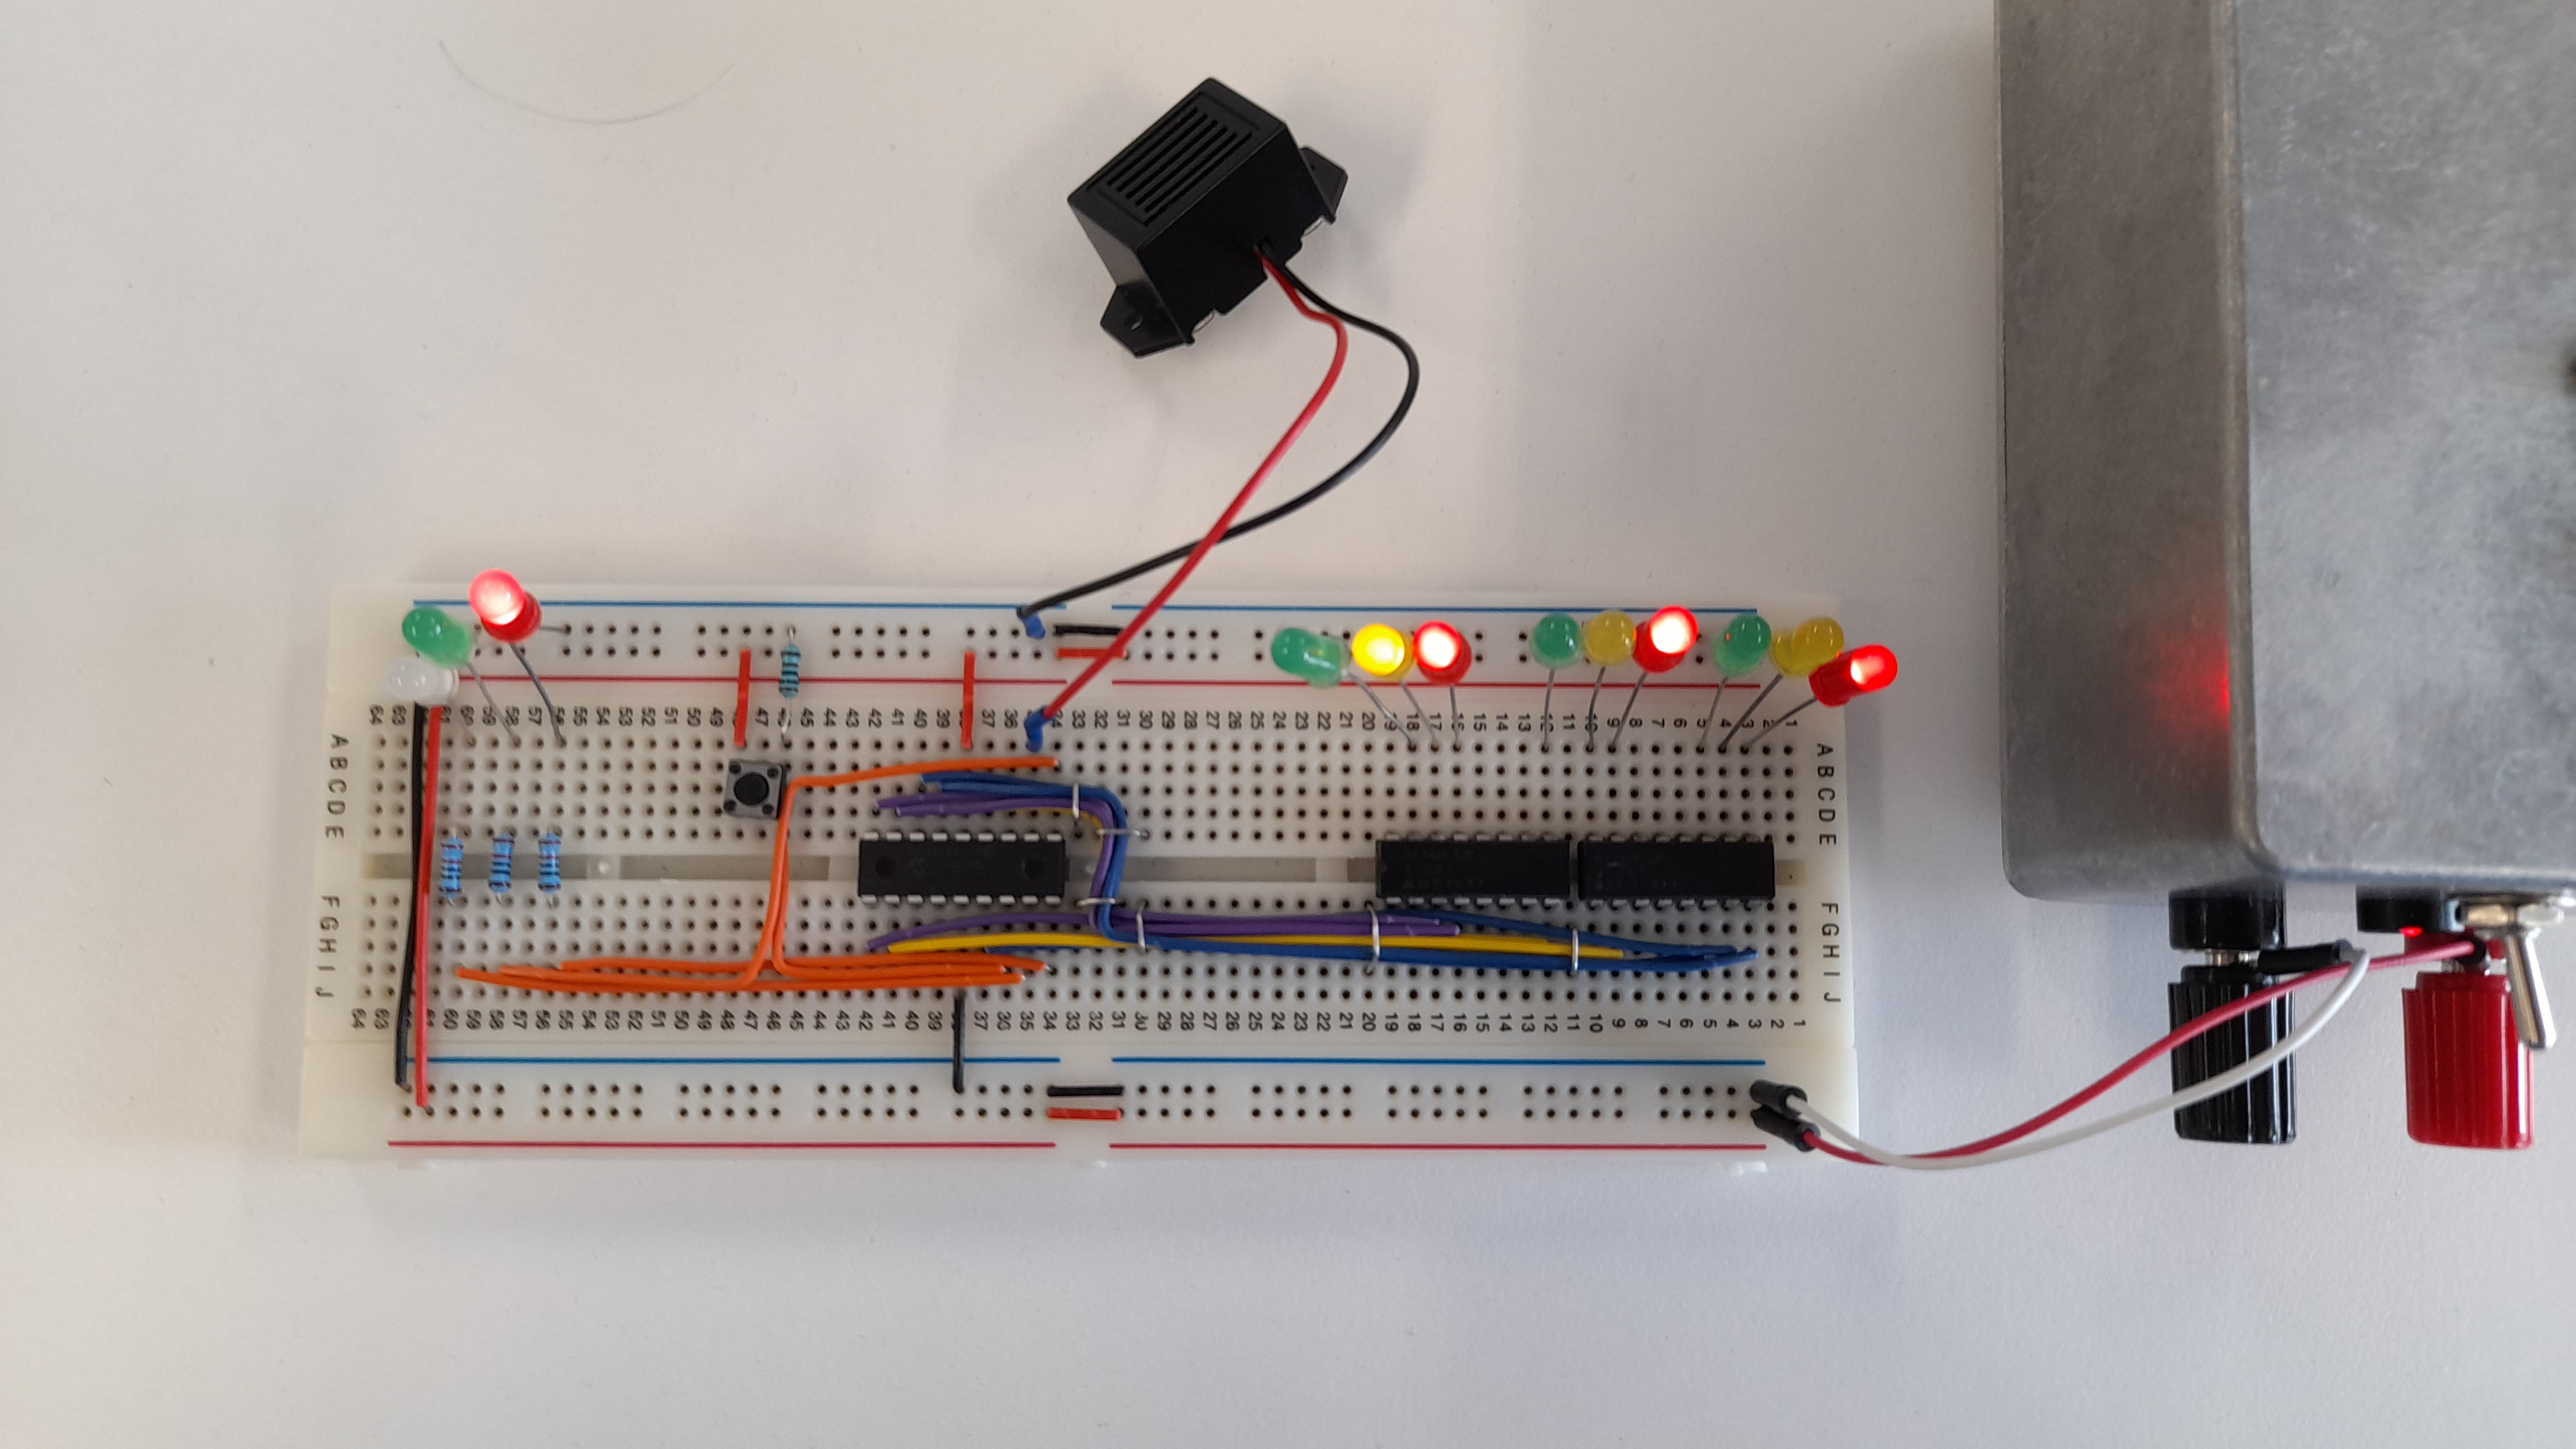
\includegraphics[width=0.9\textwidth]{images/final-testing/state_1.jpg}
        \caption{State 1 - pink traffic lights in red and amber phase}
        \label{fig:state_1}
    \end{minipage}\hfill
    \begin{minipage}{0.45\textwidth}
        \centering
        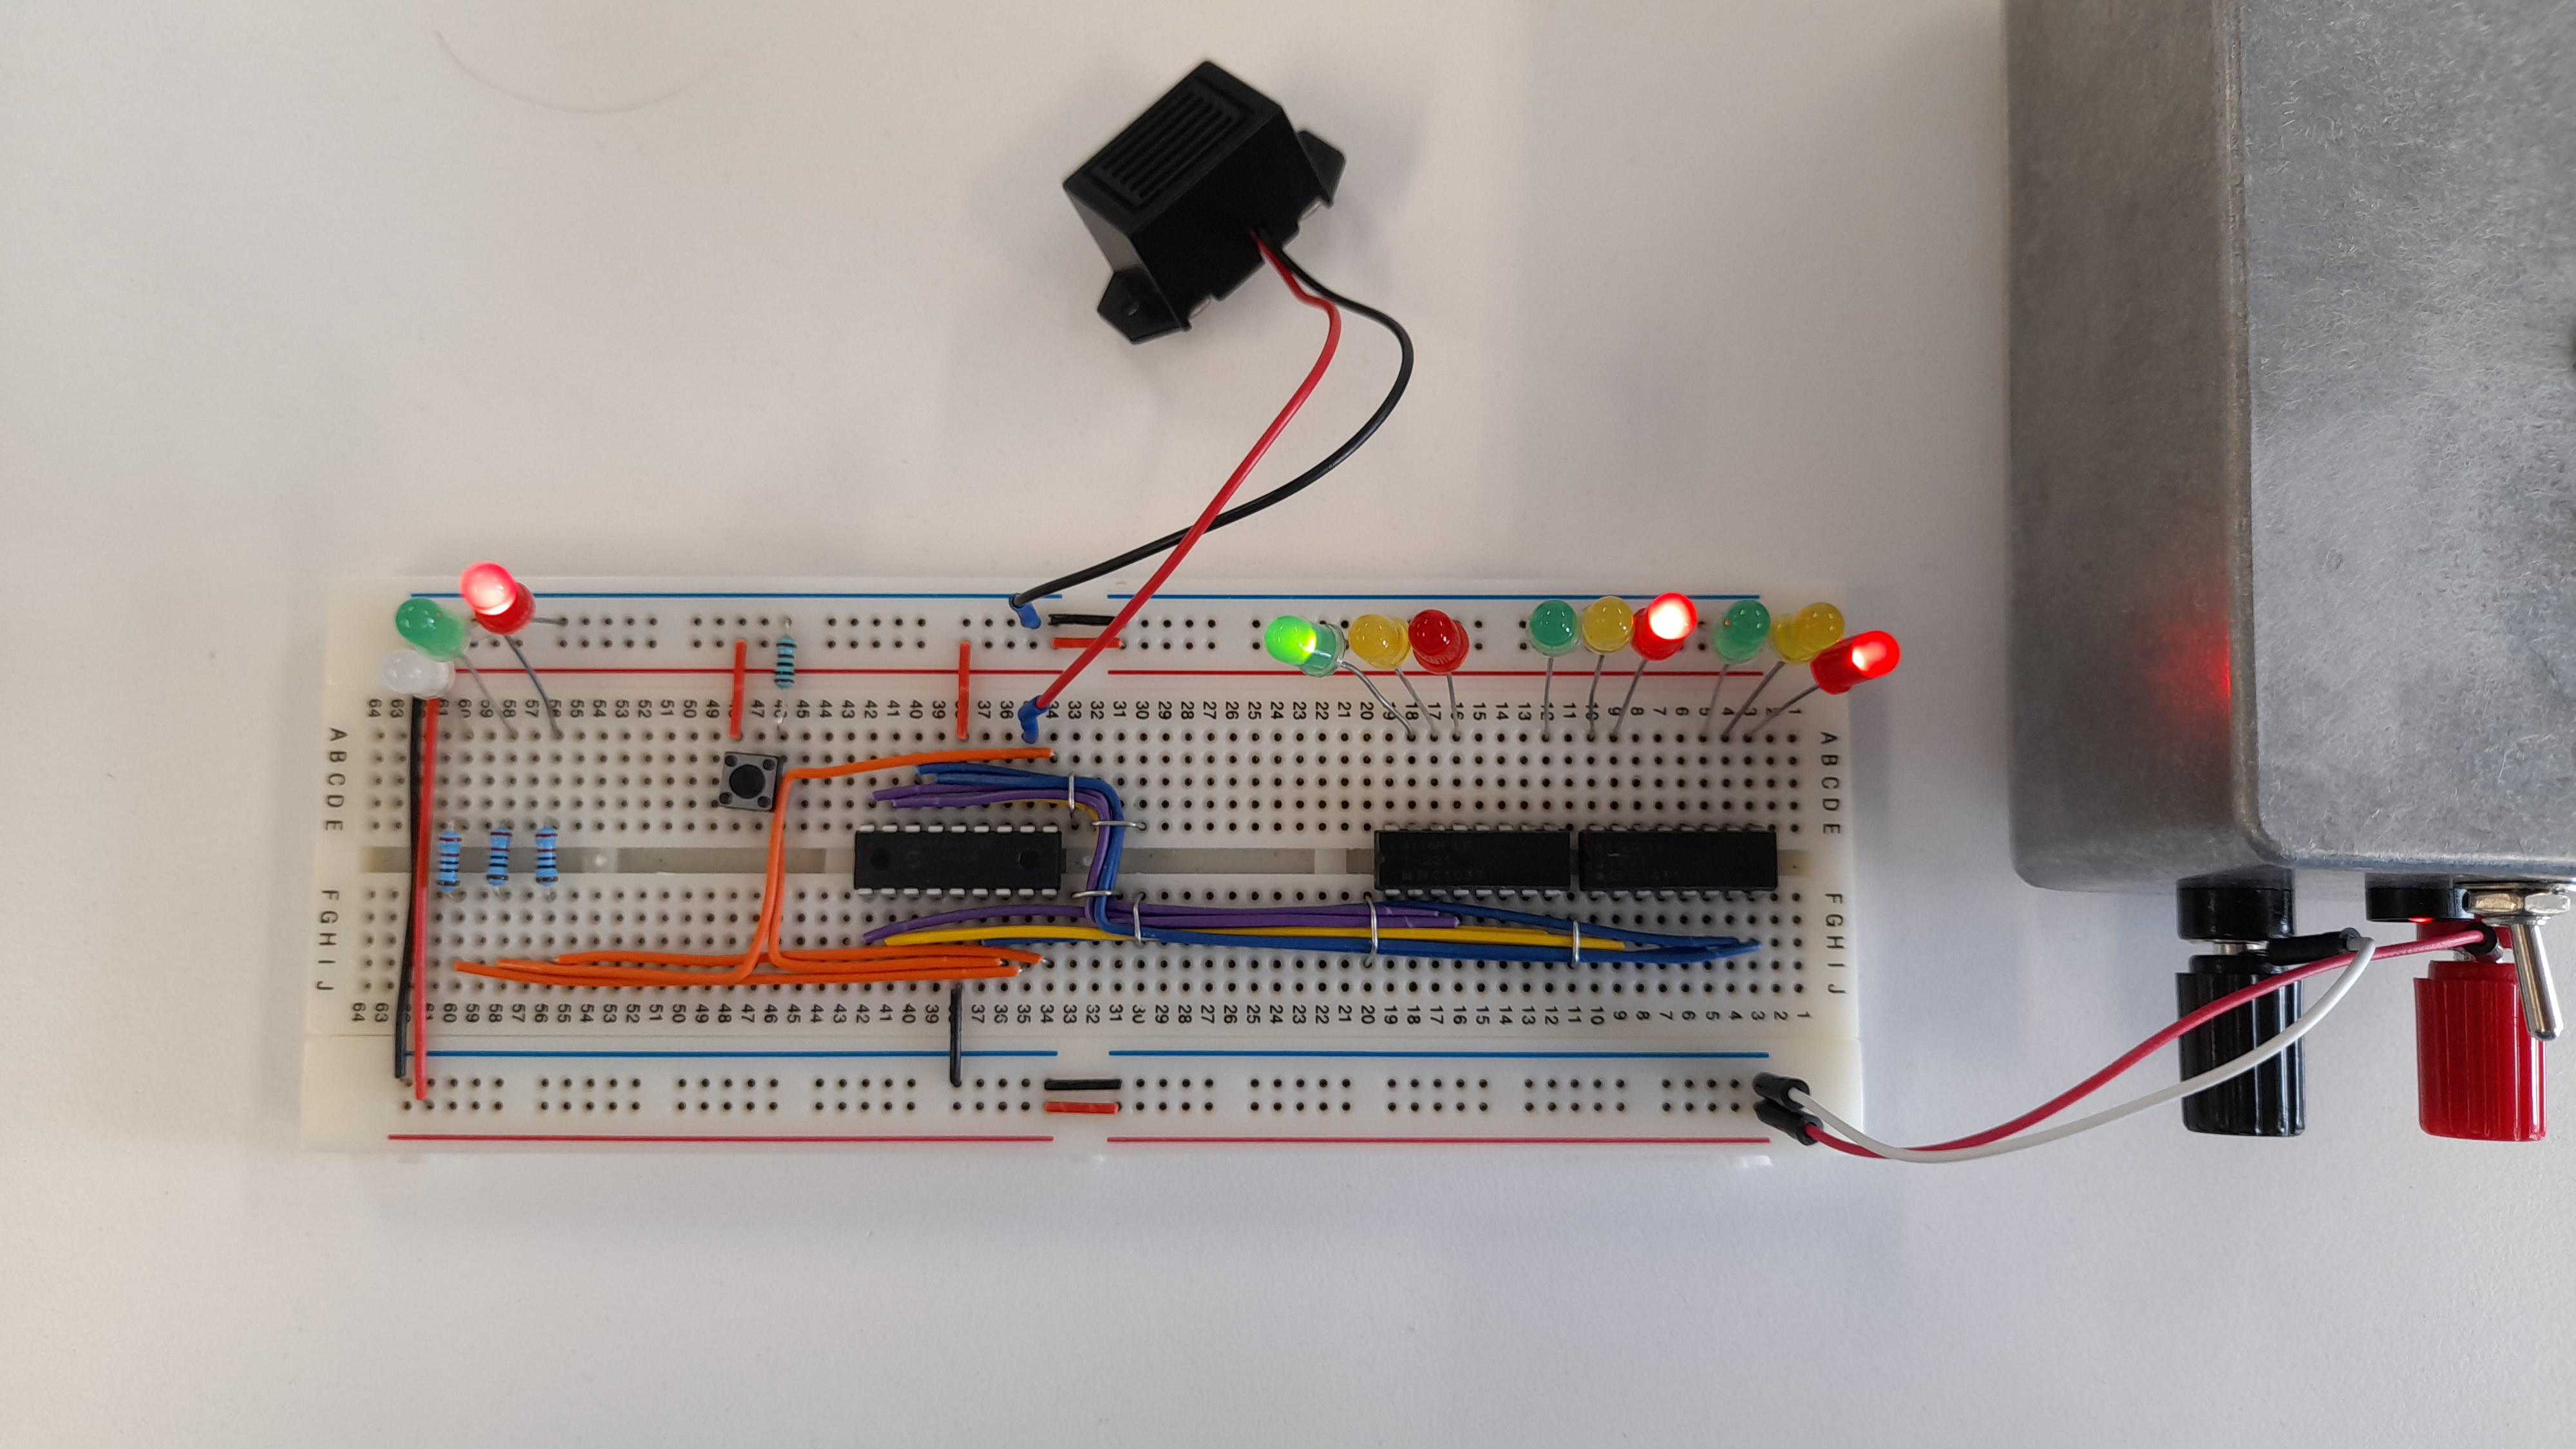
\includegraphics[width=0.9\textwidth]{images/final-testing/state_2.jpg}
        \caption{State 2 - pink traffic lights in green phase}
        \label{fig:state_2}
    \end{minipage}
\end{figure}
\begin{figure}[H]
    \begin{minipage}{0.45\textwidth}
        \centering
        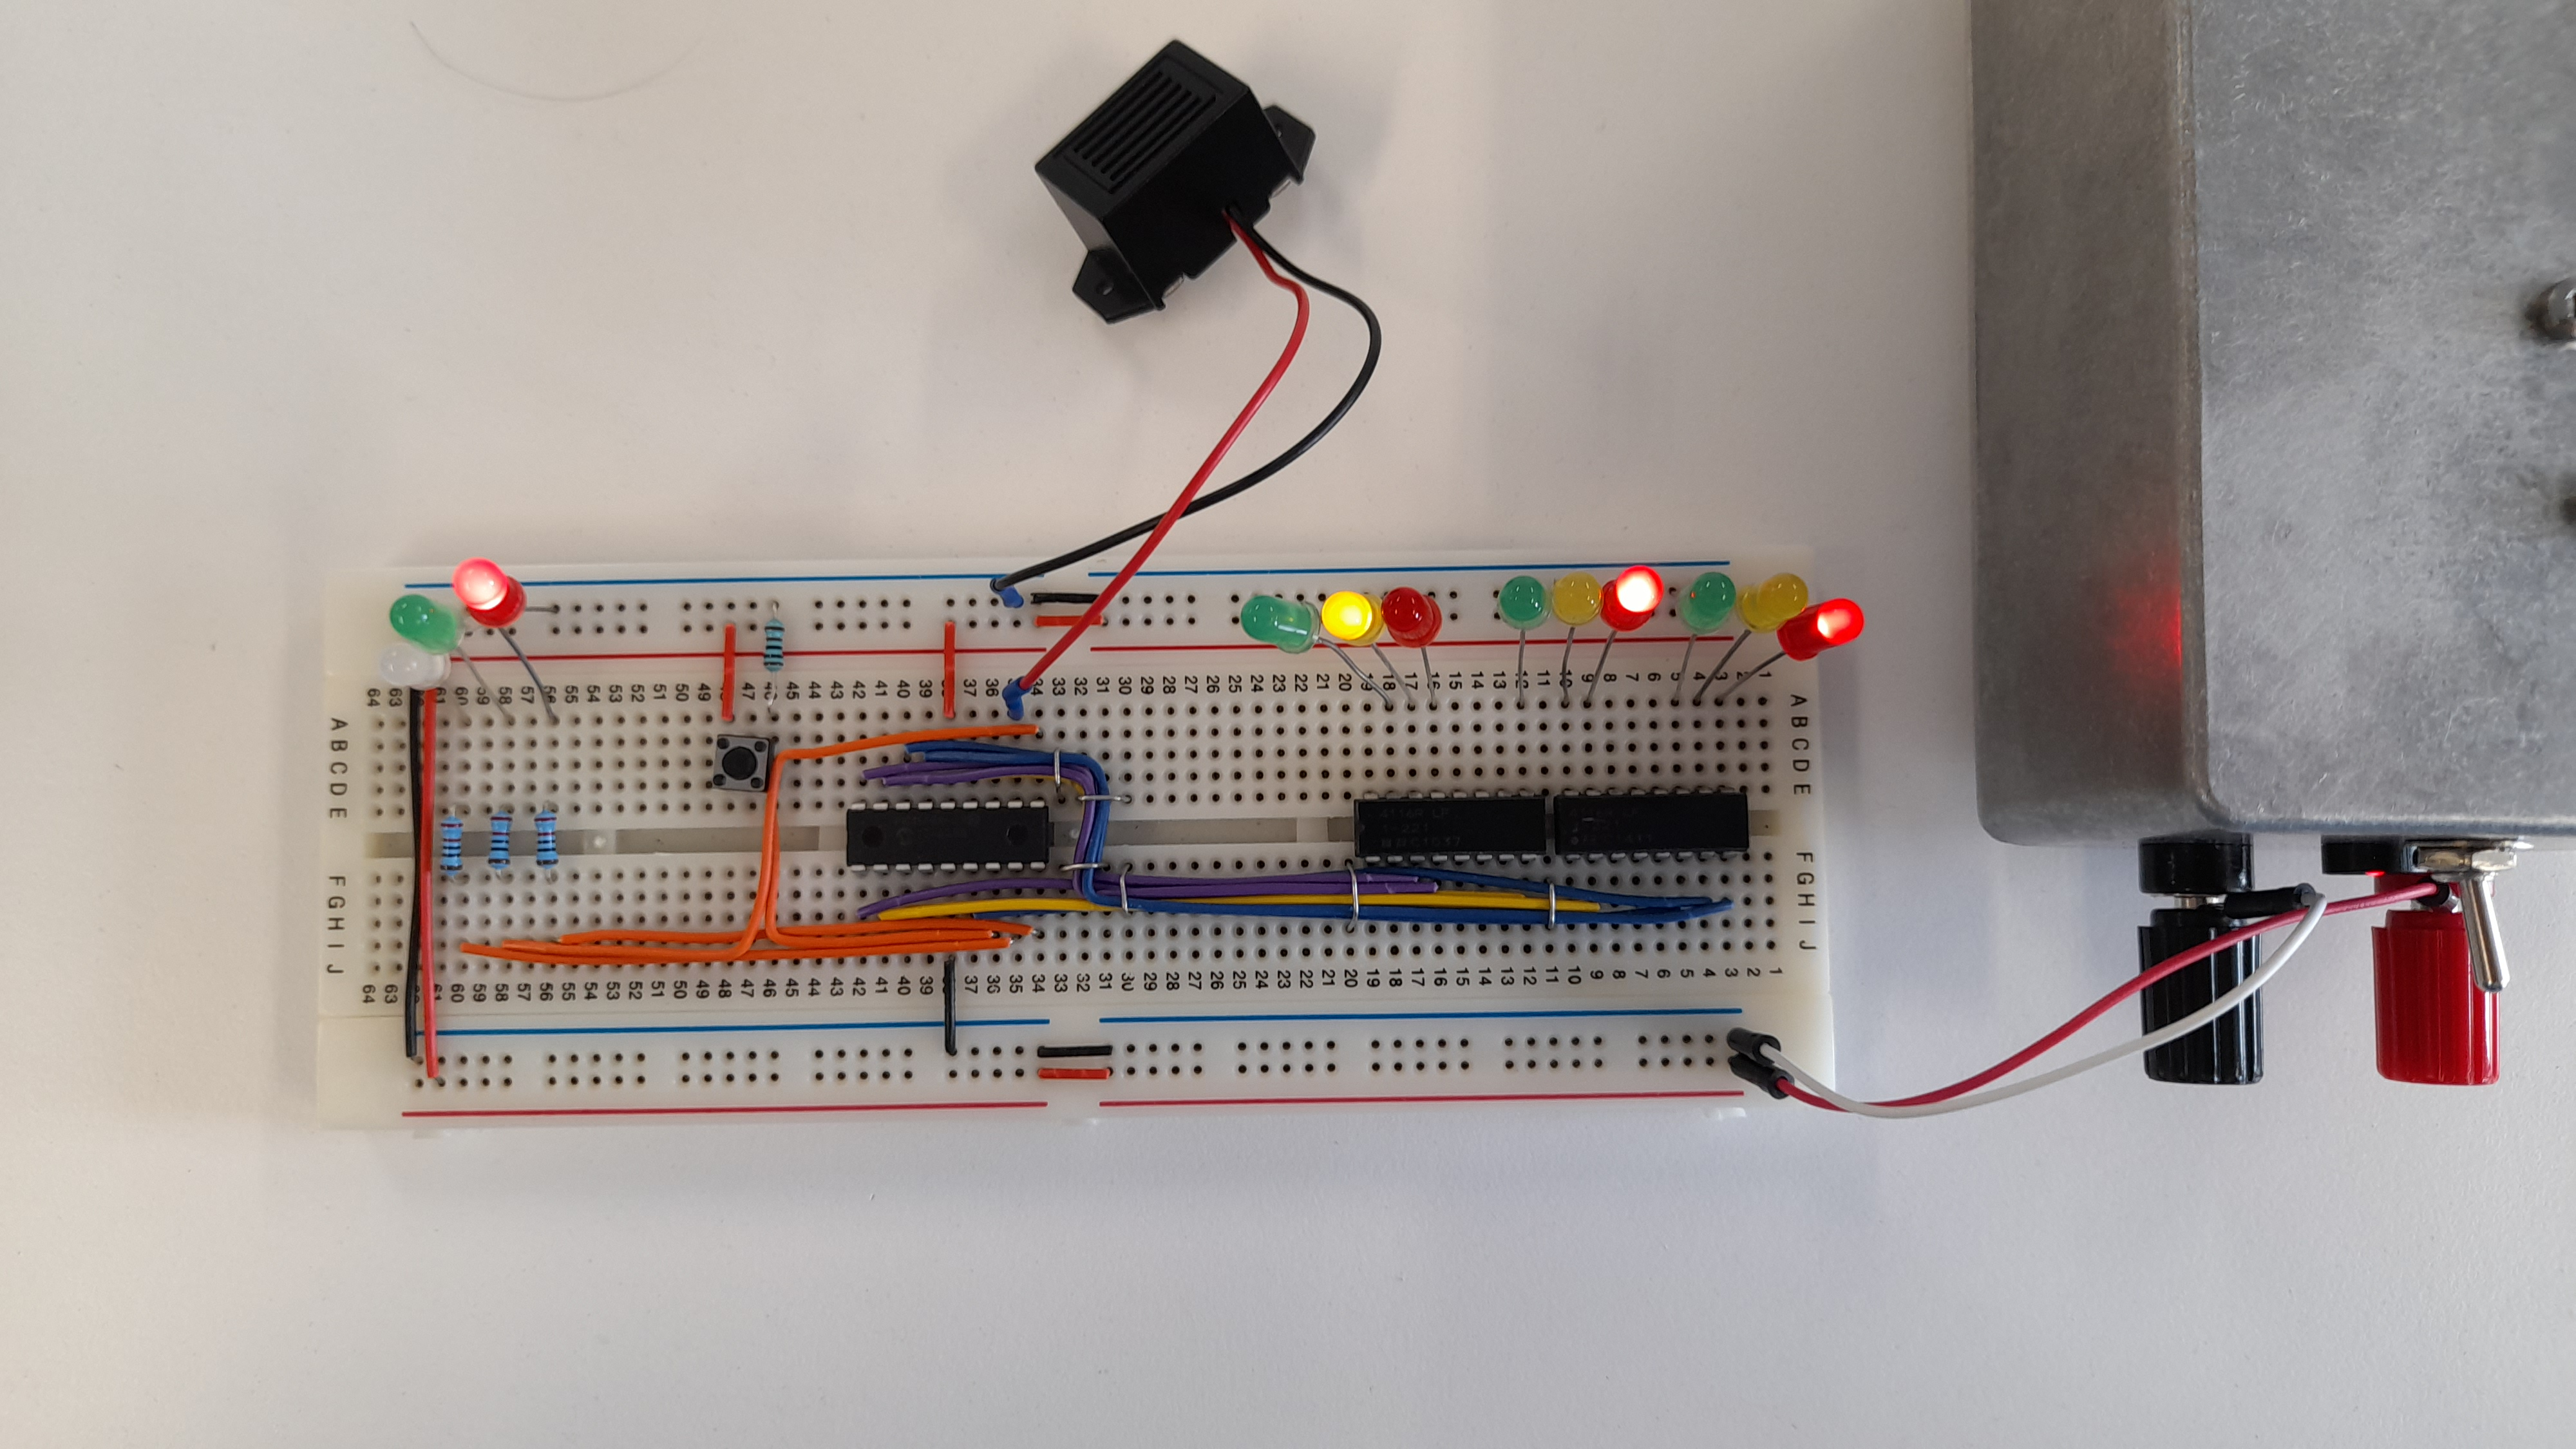
\includegraphics[width=0.9\textwidth]{images/final-testing/state_3.jpg}
        \caption{State 3 - pink traffic lights in amber phase}
        \label{fig:state_3}
    \end{minipage}\hfill
    \begin{minipage}{0.45\textwidth}
        \centering
        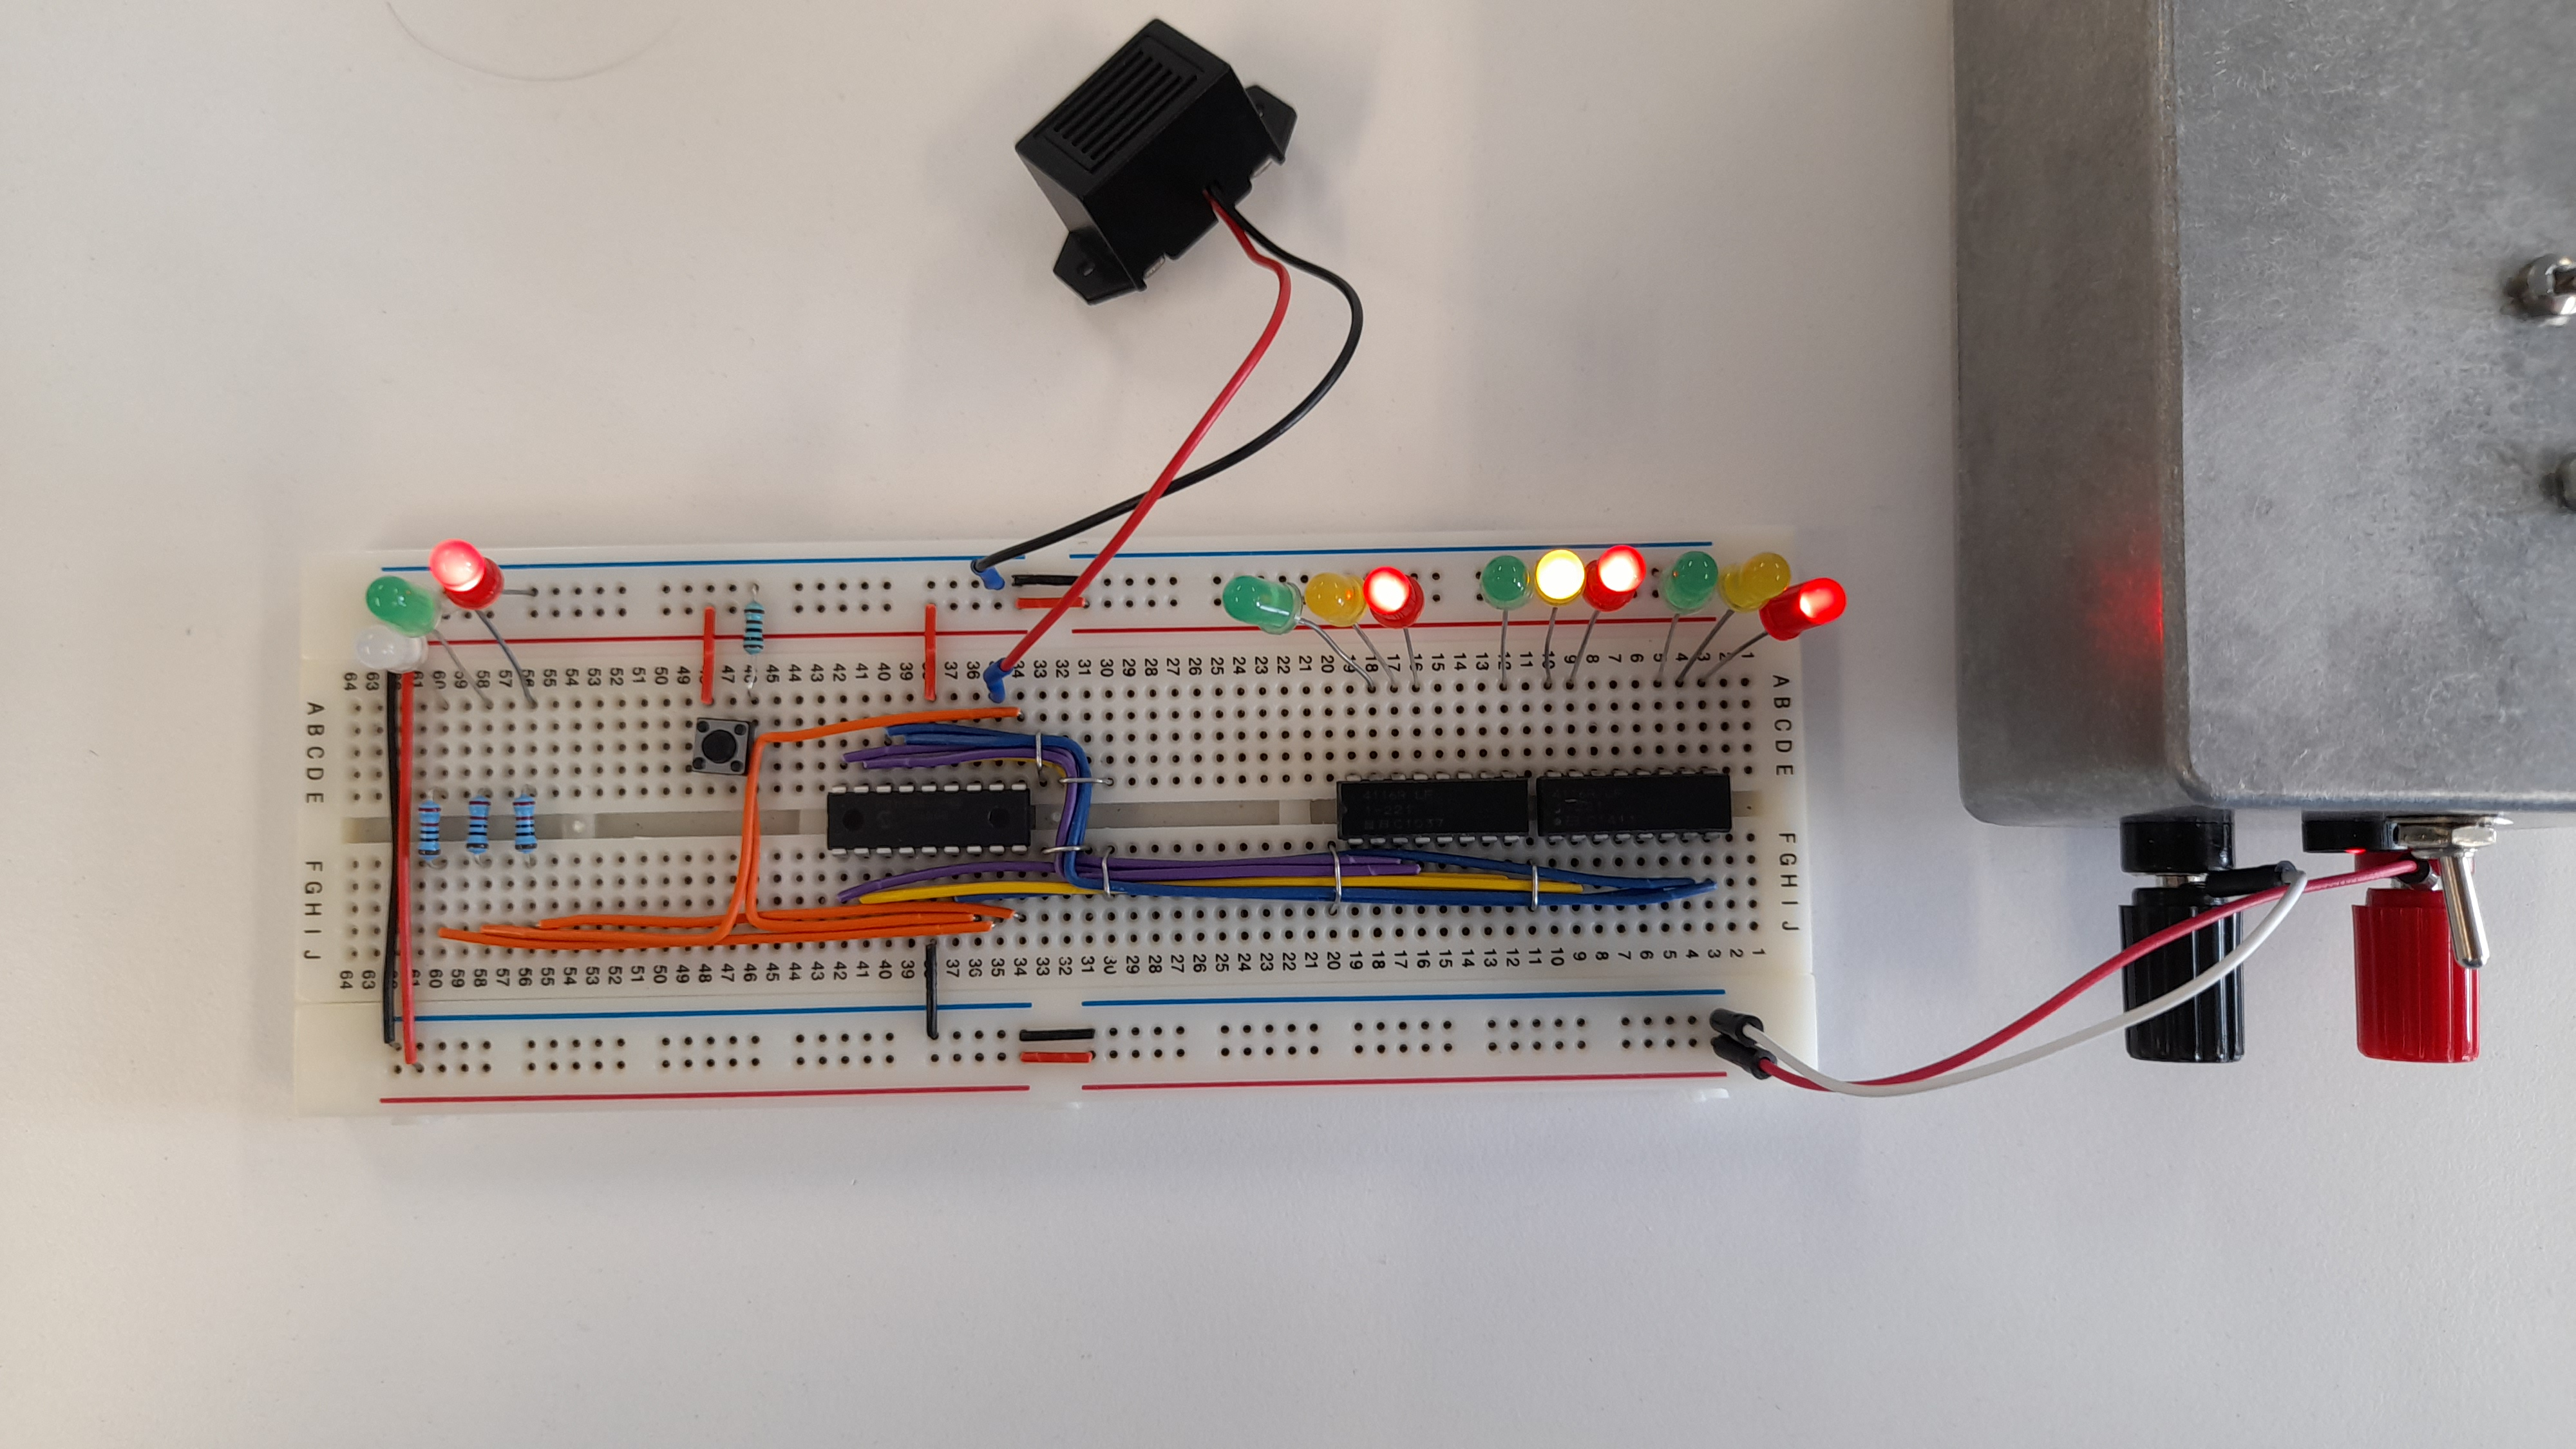
\includegraphics[width=0.9\textwidth]{images/final-testing/state_4.jpg}
        \caption{State 4 - green traffic lights in red and amber phase}
        \label{fig:state_4}
    \end{minipage}
\end{figure}
\begin{figure}[H]
    \begin{minipage}{0.45\textwidth}
        \centering
        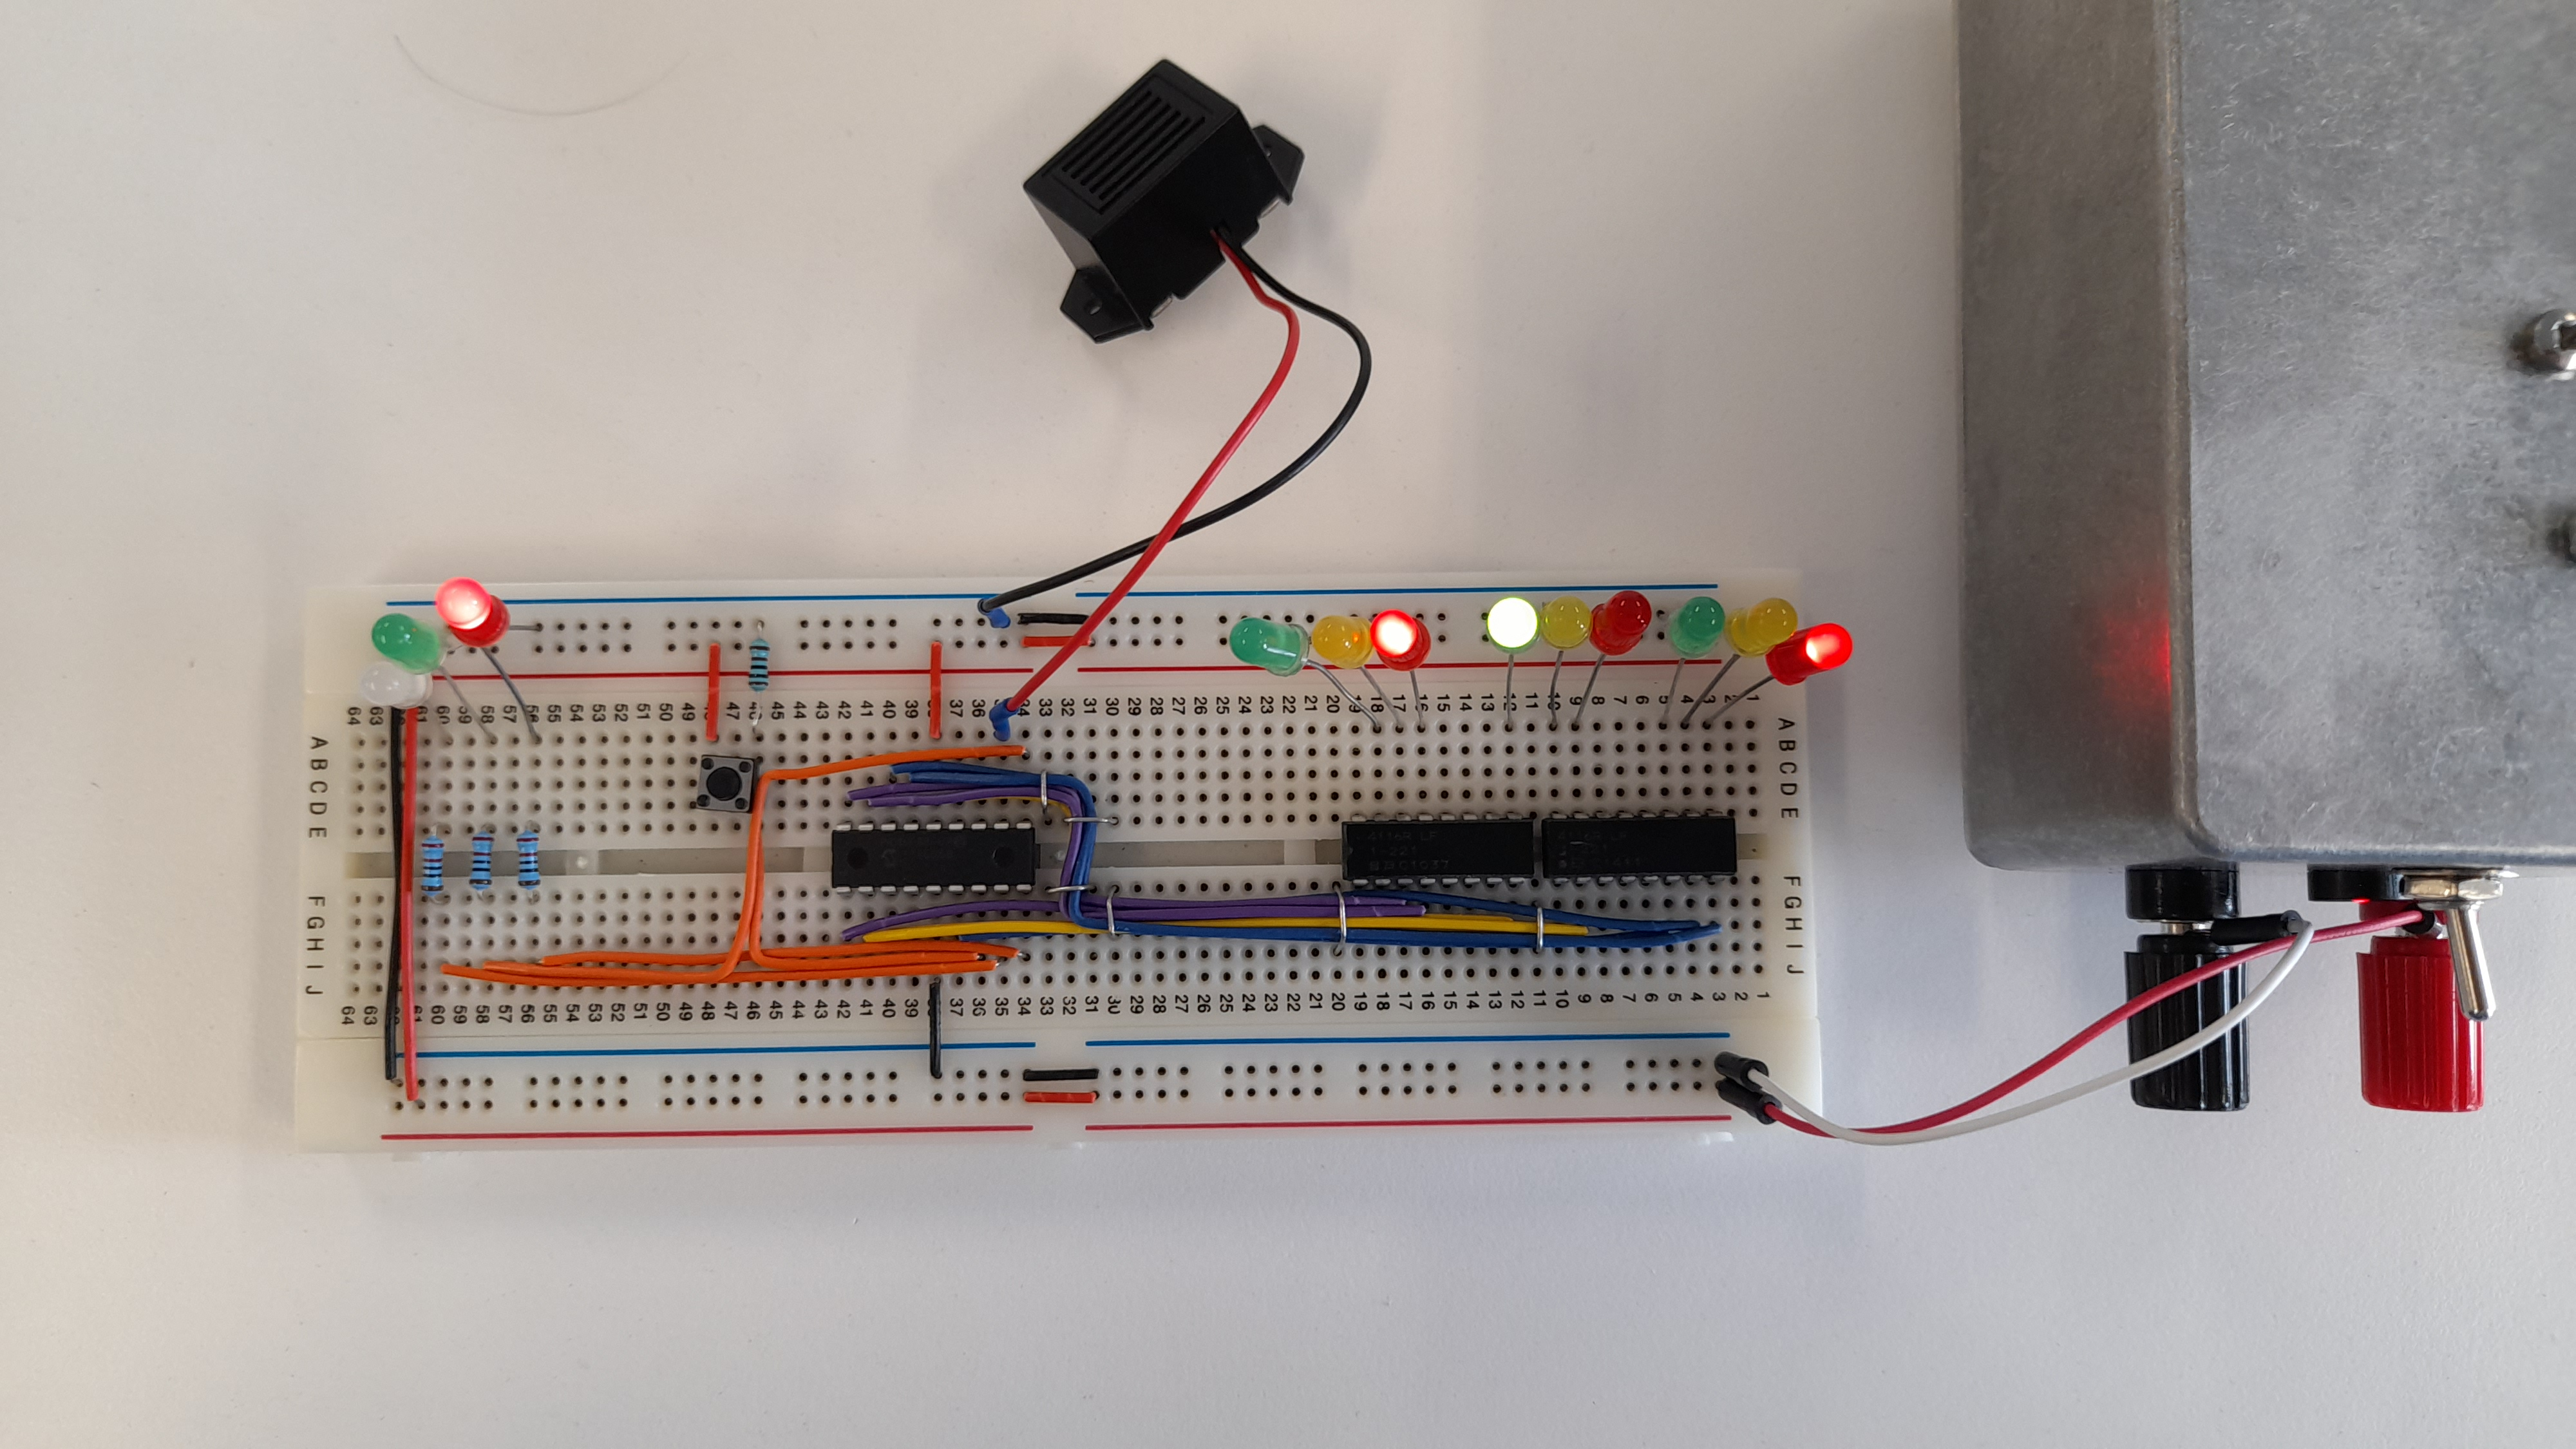
\includegraphics[width=0.9\textwidth]{images/final-testing/state_5.jpg}
        \caption{State 5 - green traffic lights in green phase}
        \label{fig:state_5}
    \end{minipage}\hfill
    \begin{minipage}{0.45\textwidth}
        \centering
        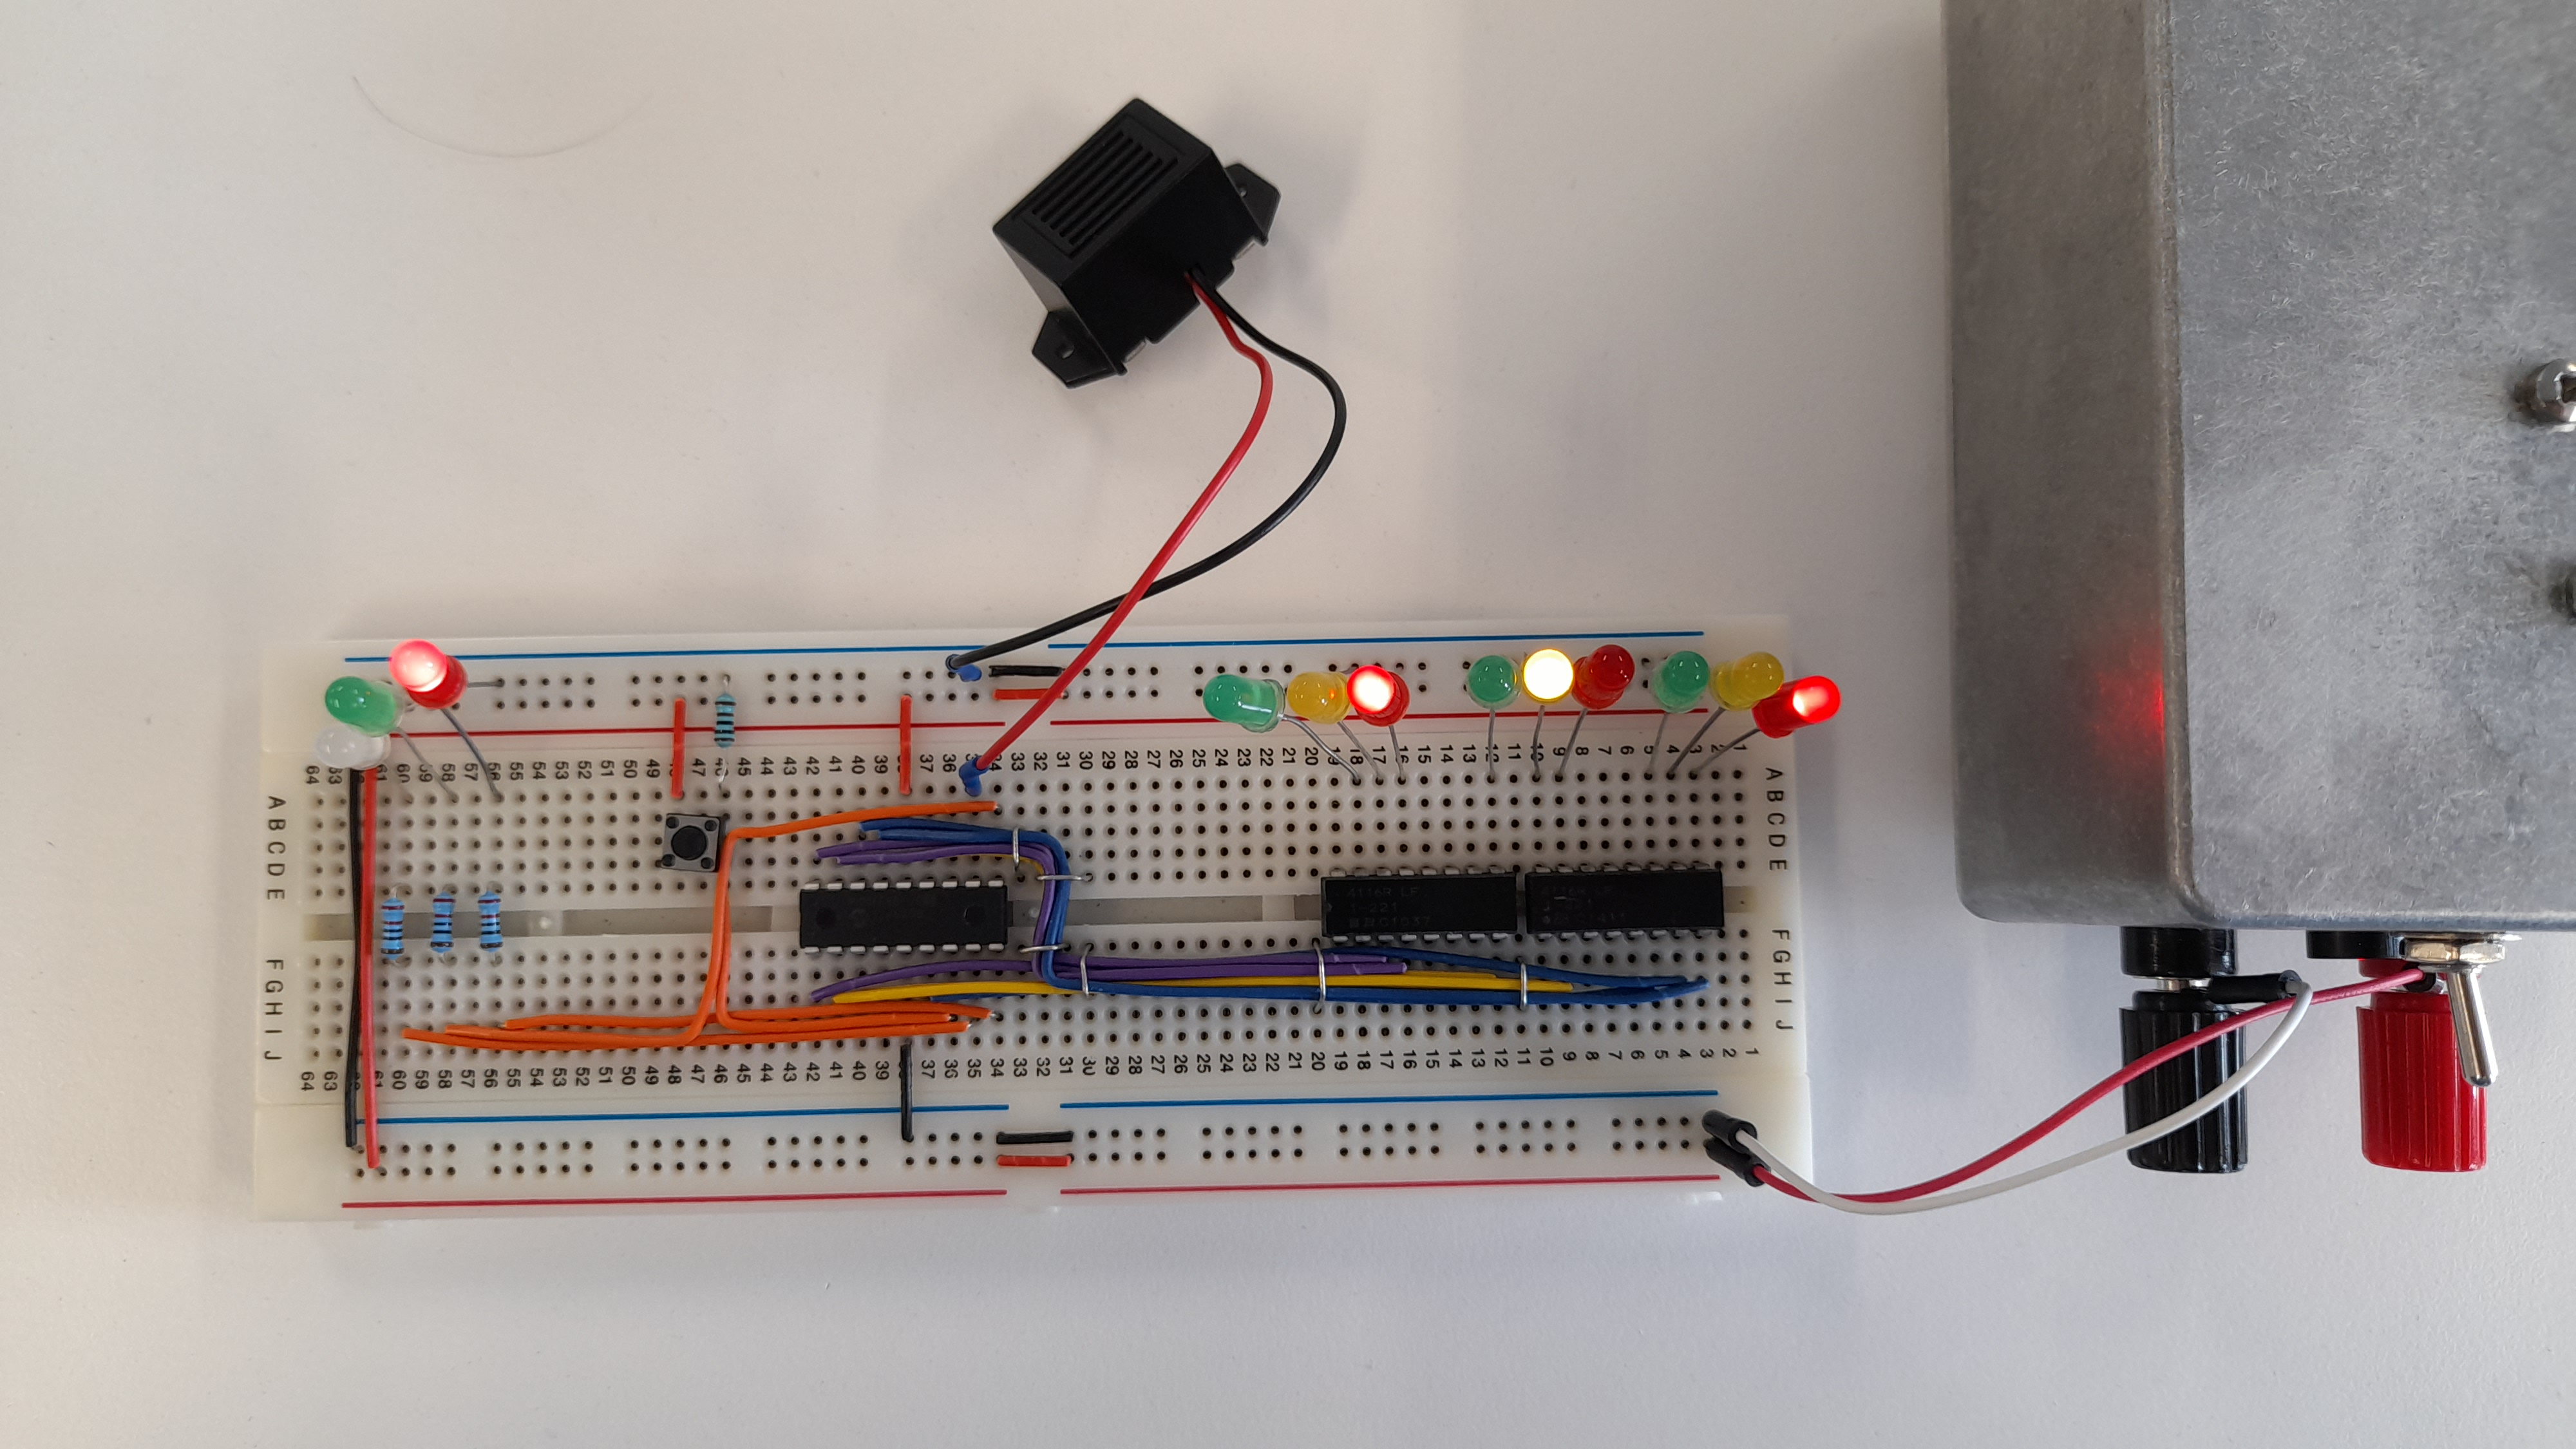
\includegraphics[width=0.9\textwidth]{images/final-testing/state_6.jpg}
        \caption{State 6 - green traffic lights in amber phase}
        \label{fig:state_6}
    \end{minipage}
\end{figure}
\begin{figure}[H]
    \begin{minipage}{0.45\textwidth}
        \centering
        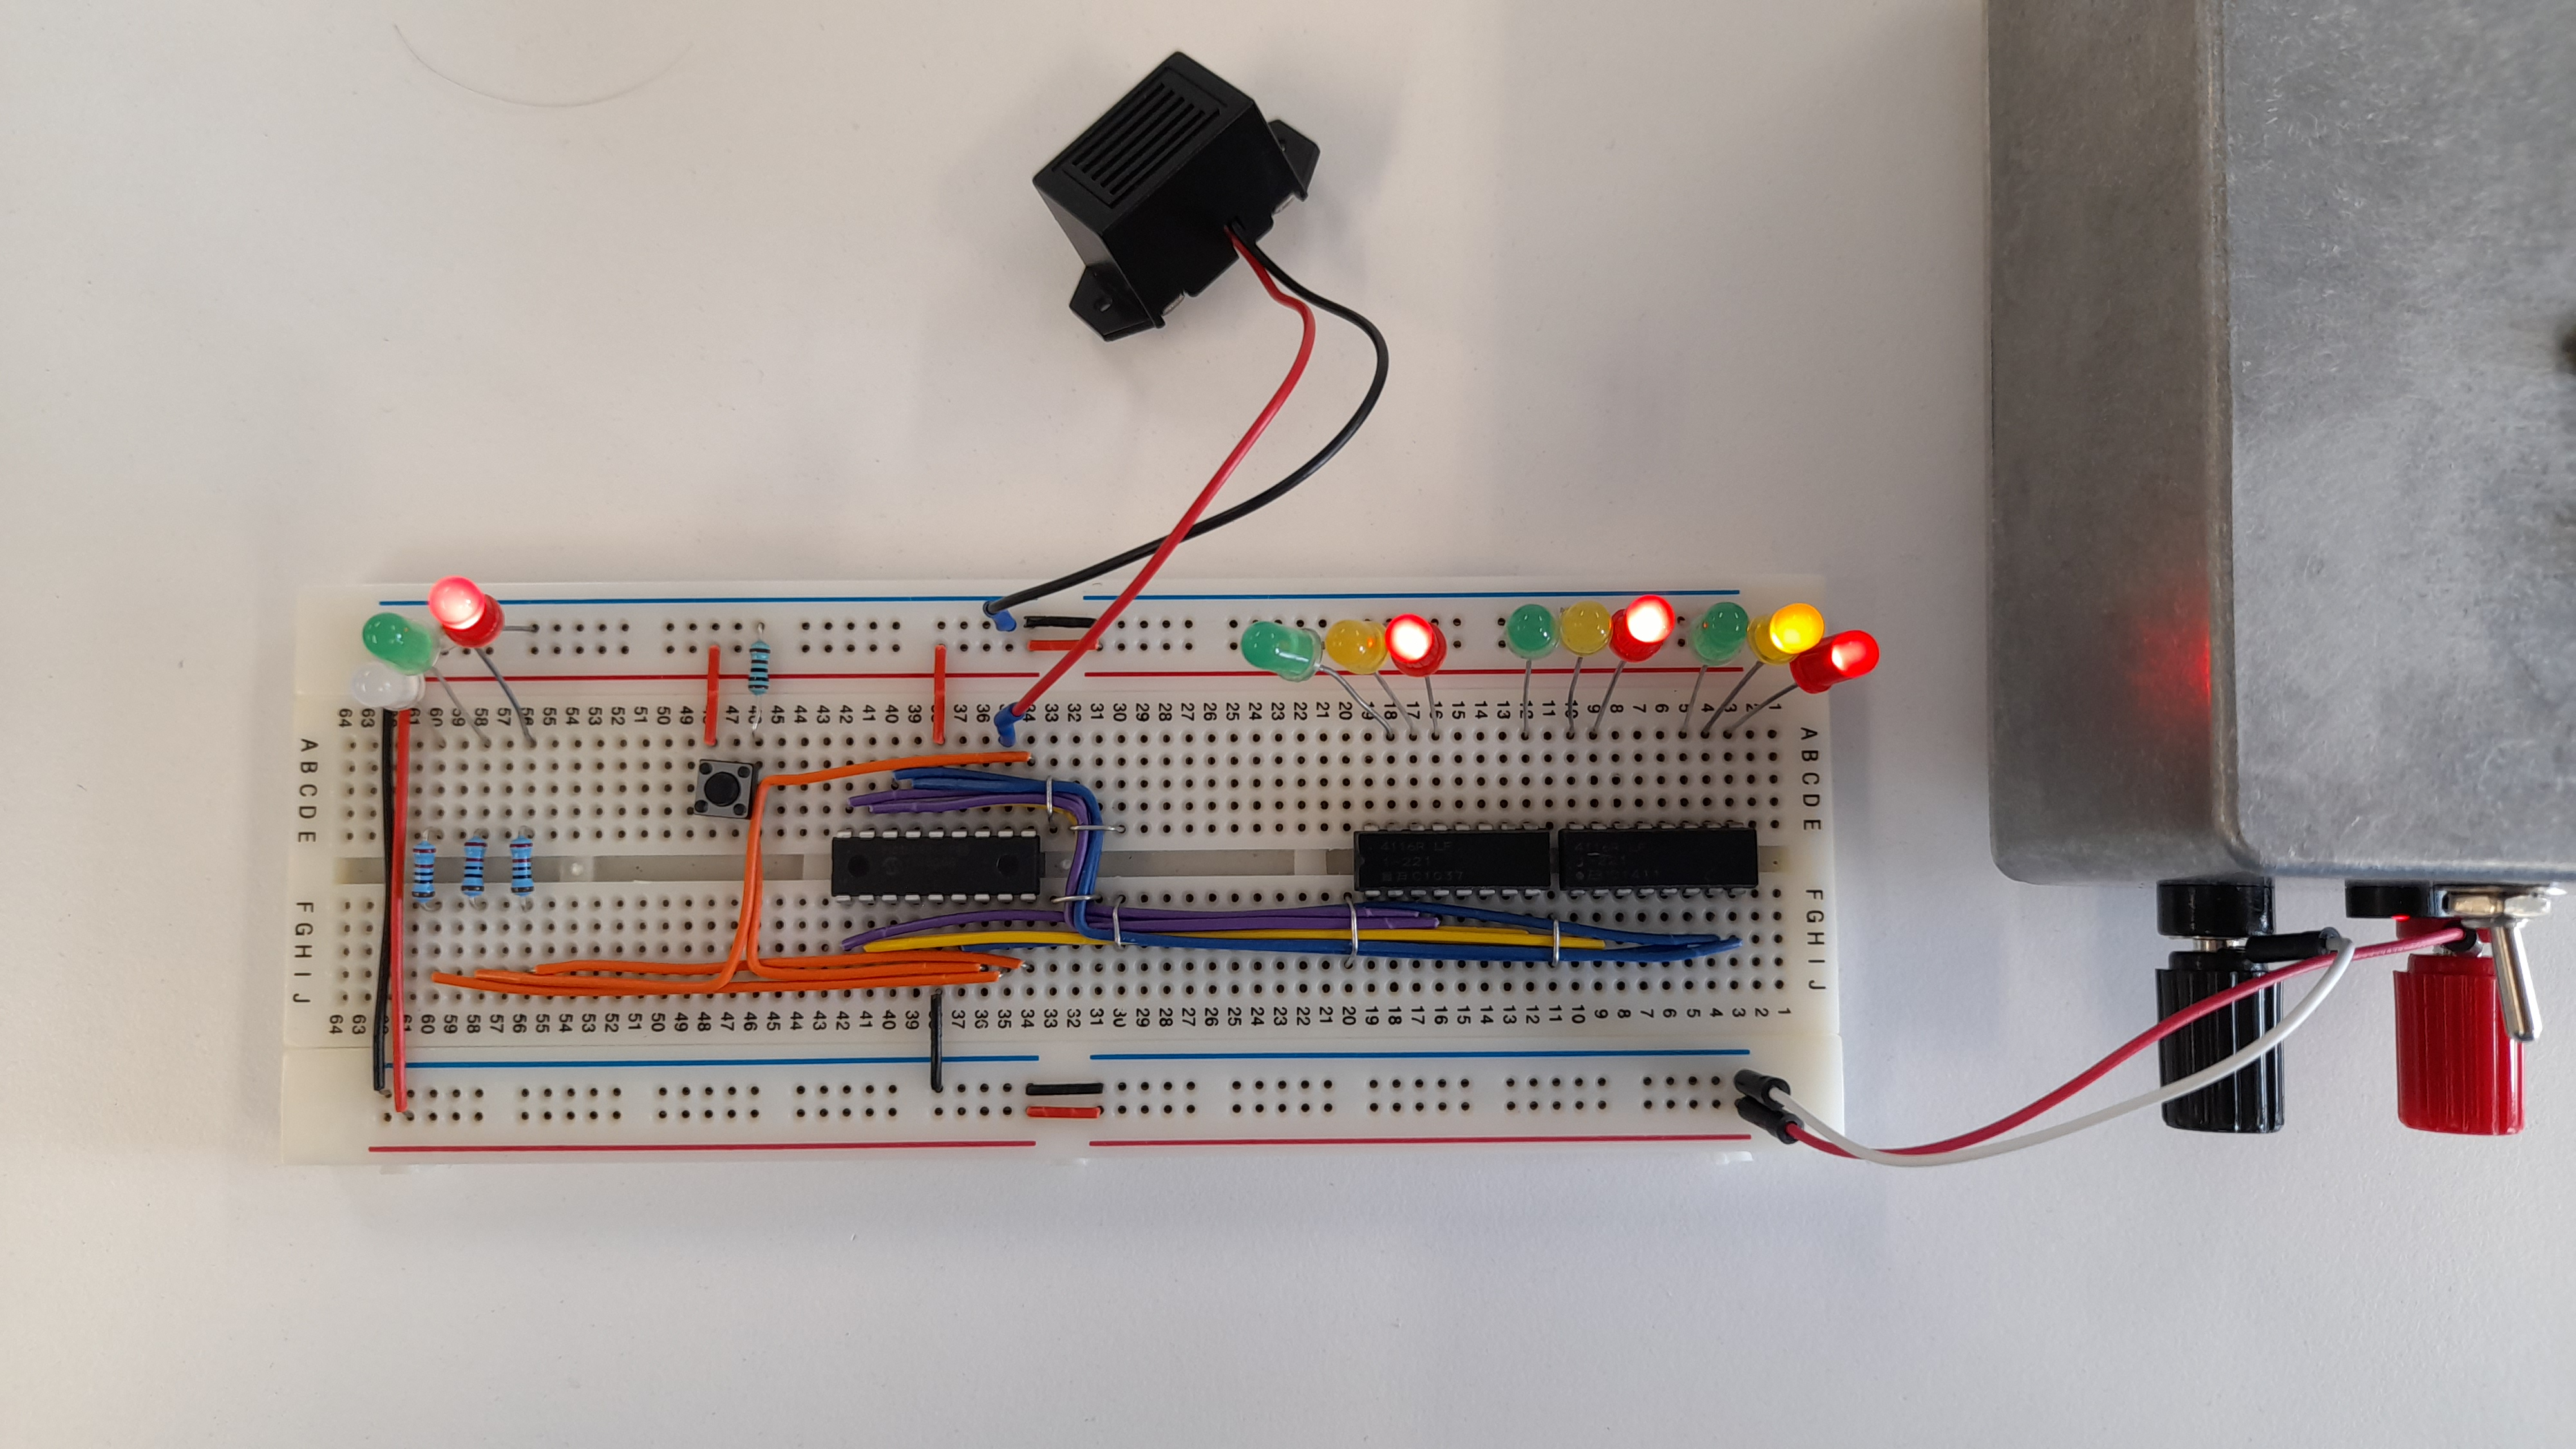
\includegraphics[width=0.9\textwidth]{images/final-testing/state_7.jpg}
        \caption{State 7 - blue traffic lights in red and amber phase}
        \label{fig:state_7}
    \end{minipage}\hfill
    \begin{minipage}{0.45\textwidth}
        \centering
        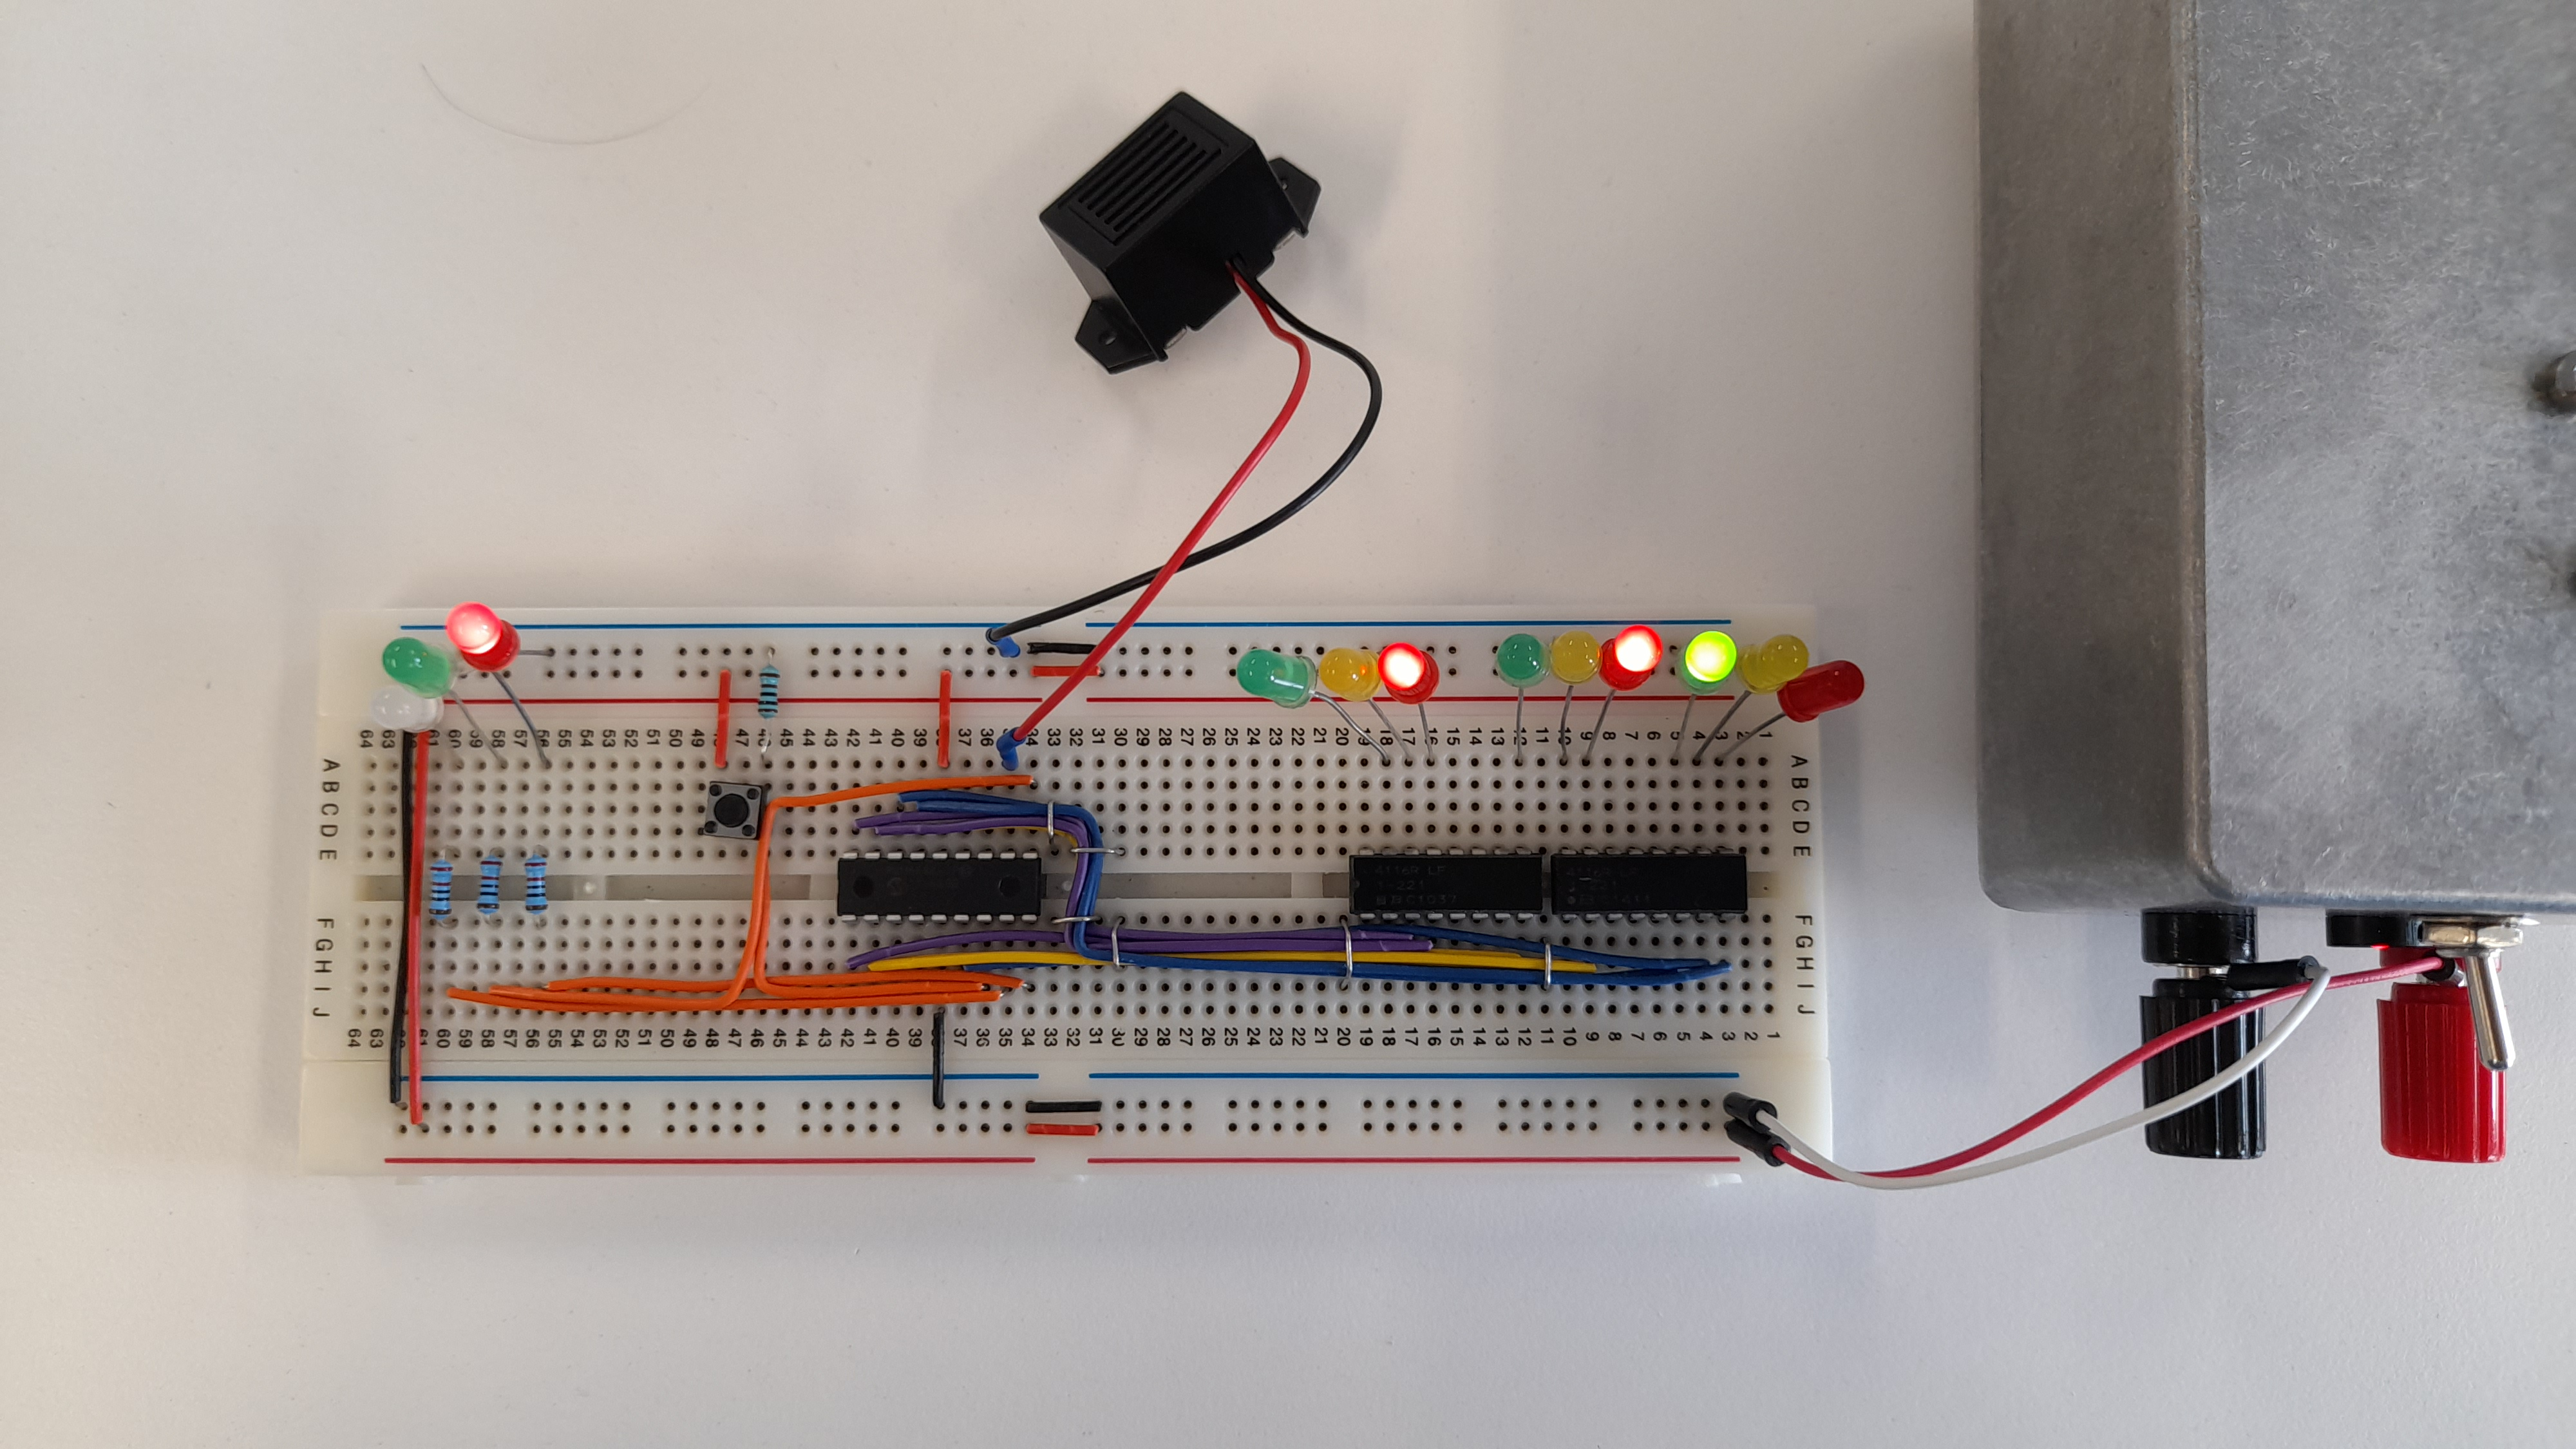
\includegraphics[width=0.9\textwidth]{images/final-testing/state_8.jpg}
        \caption{State 8 - blue traffic lights in green phase}
        \label{fig:state_8}
    \end{minipage}
\end{figure}
\begin{figure}[H]
    \begin{minipage}{0.45\textwidth}
        \centering
        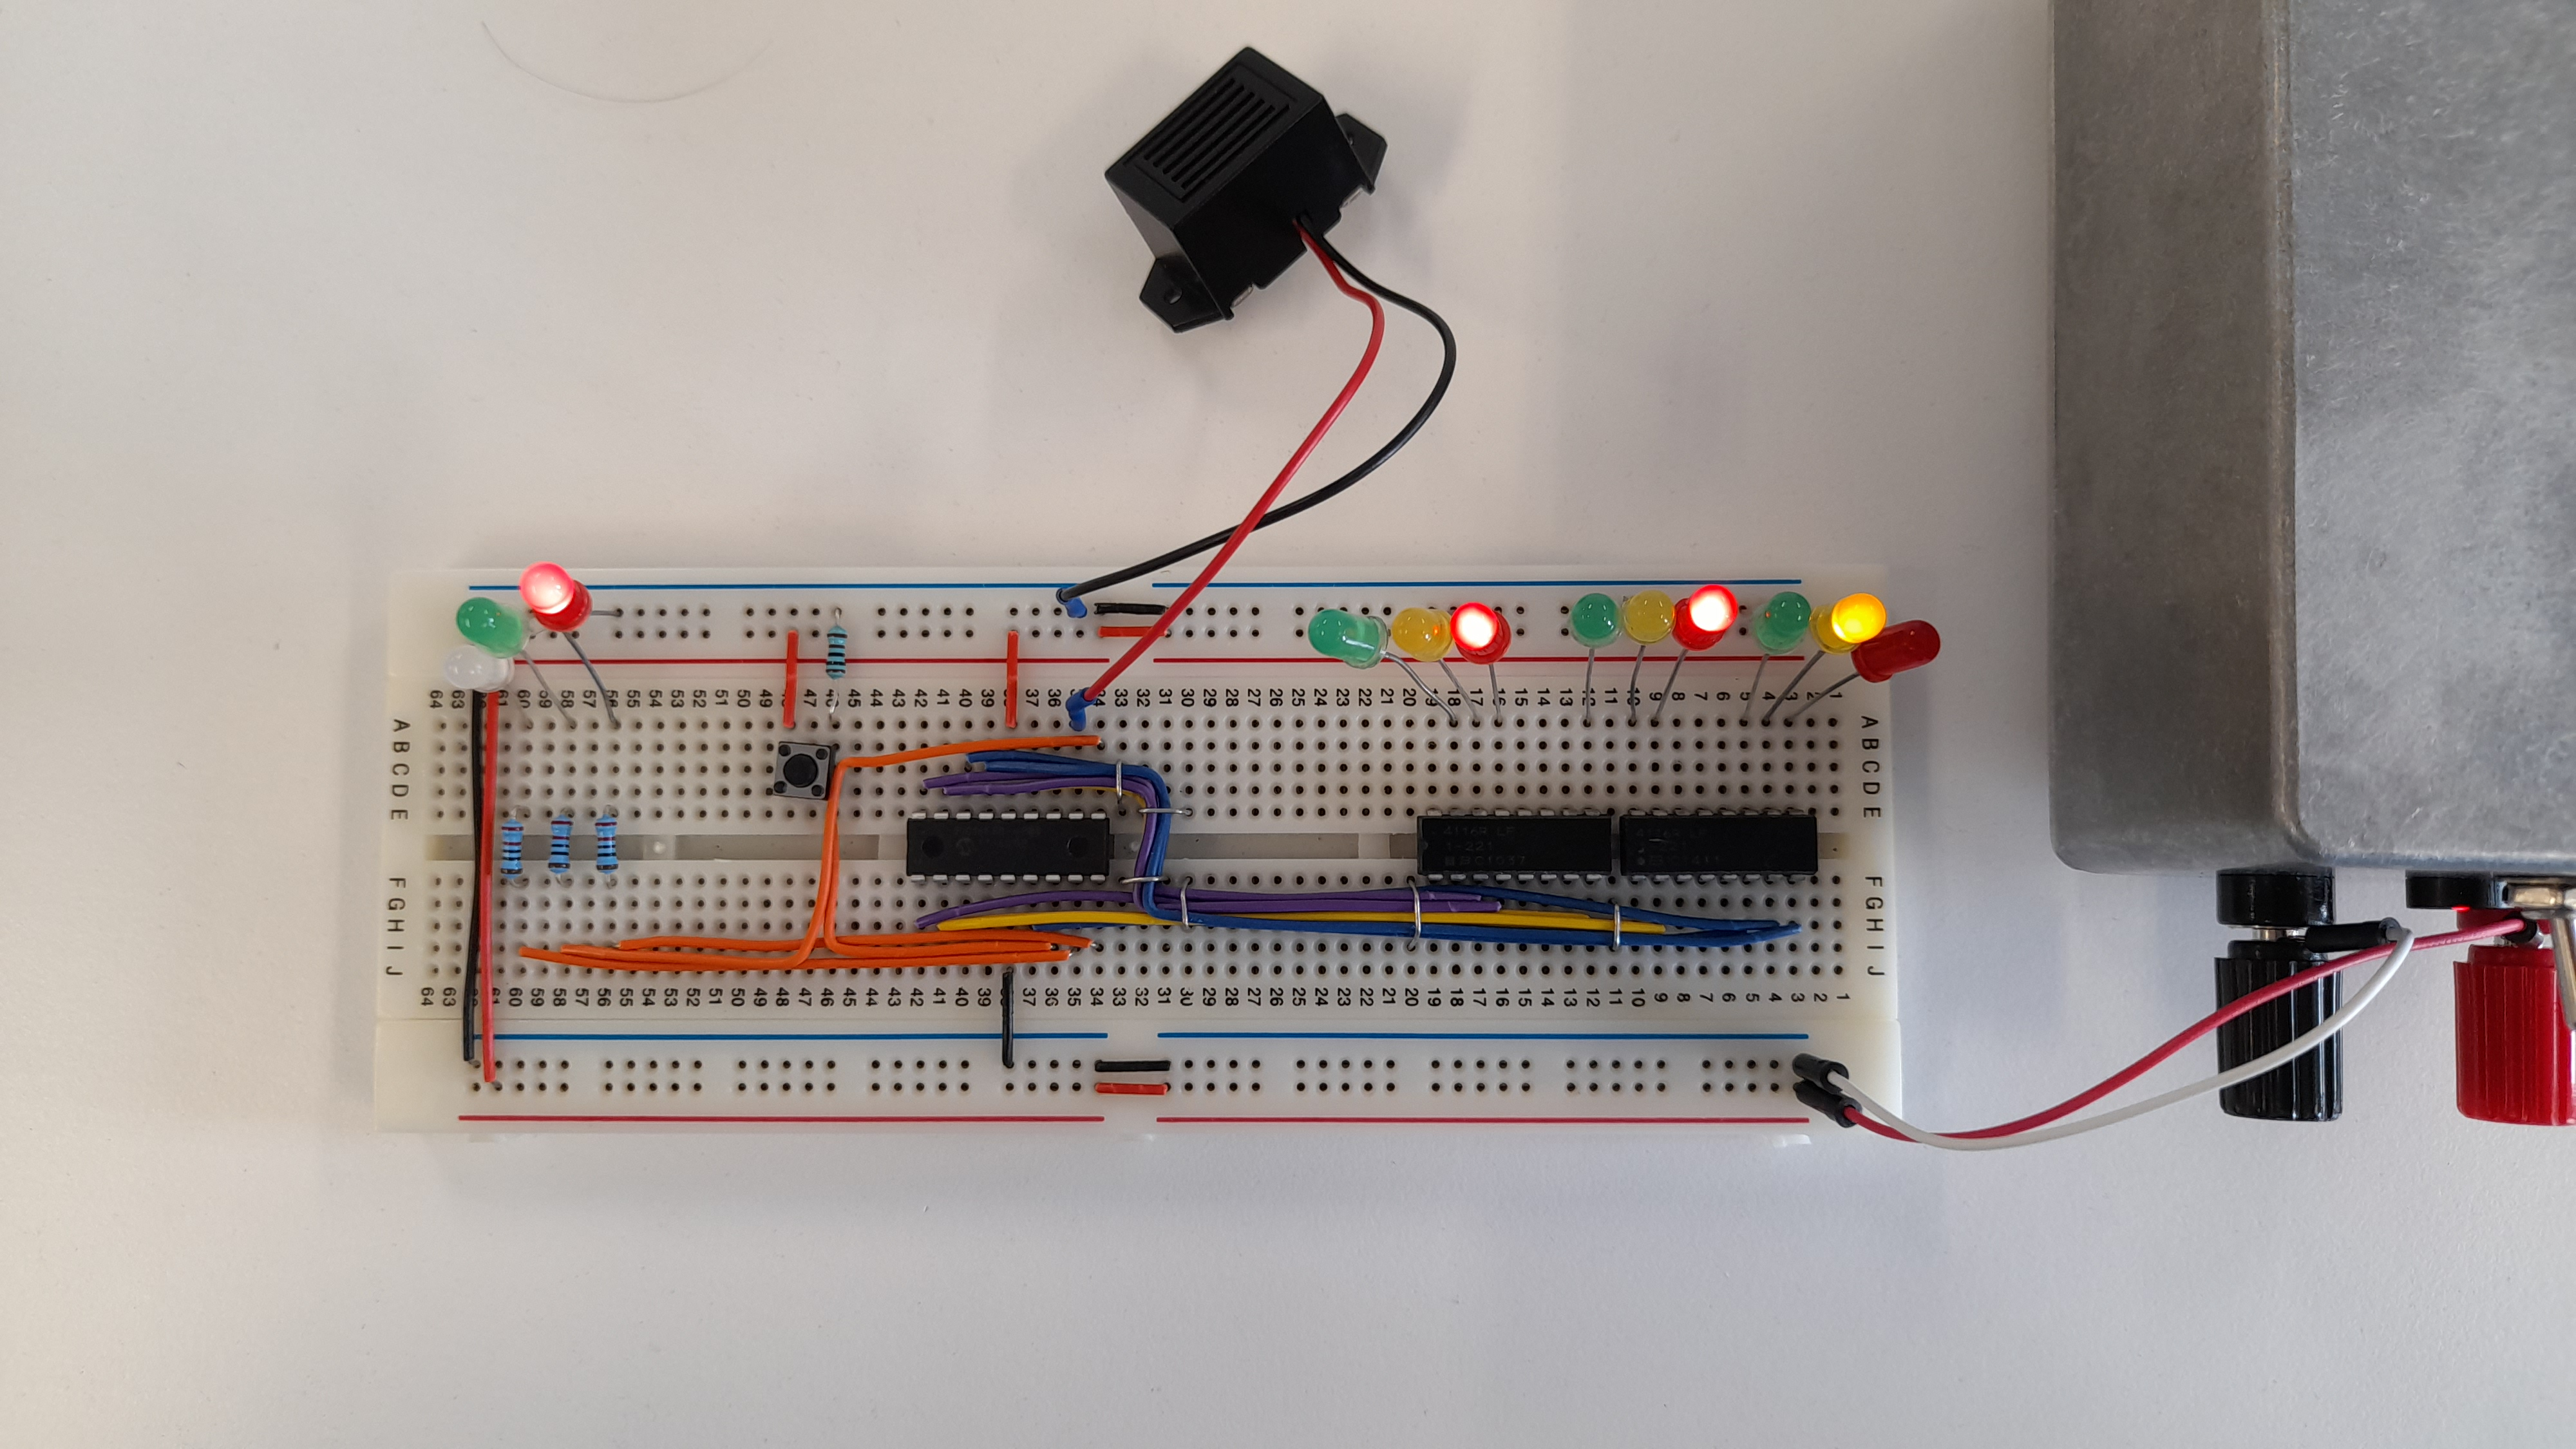
\includegraphics[width=0.9\textwidth]{images/final-testing/state_9.jpg}
        \caption{State 9 - blue traffic lights in amber phase}
        \label{fig:state_9}
    \end{minipage}\hfill
    \begin{minipage}{0.45\textwidth}
        \centering
        The system then loops back to state 1.
    \end{minipage}
\end{figure}

\subsection{Crossing Sequence}
\begin{figure}[H]
    \begin{minipage}{0.45\textwidth}
        \centering
        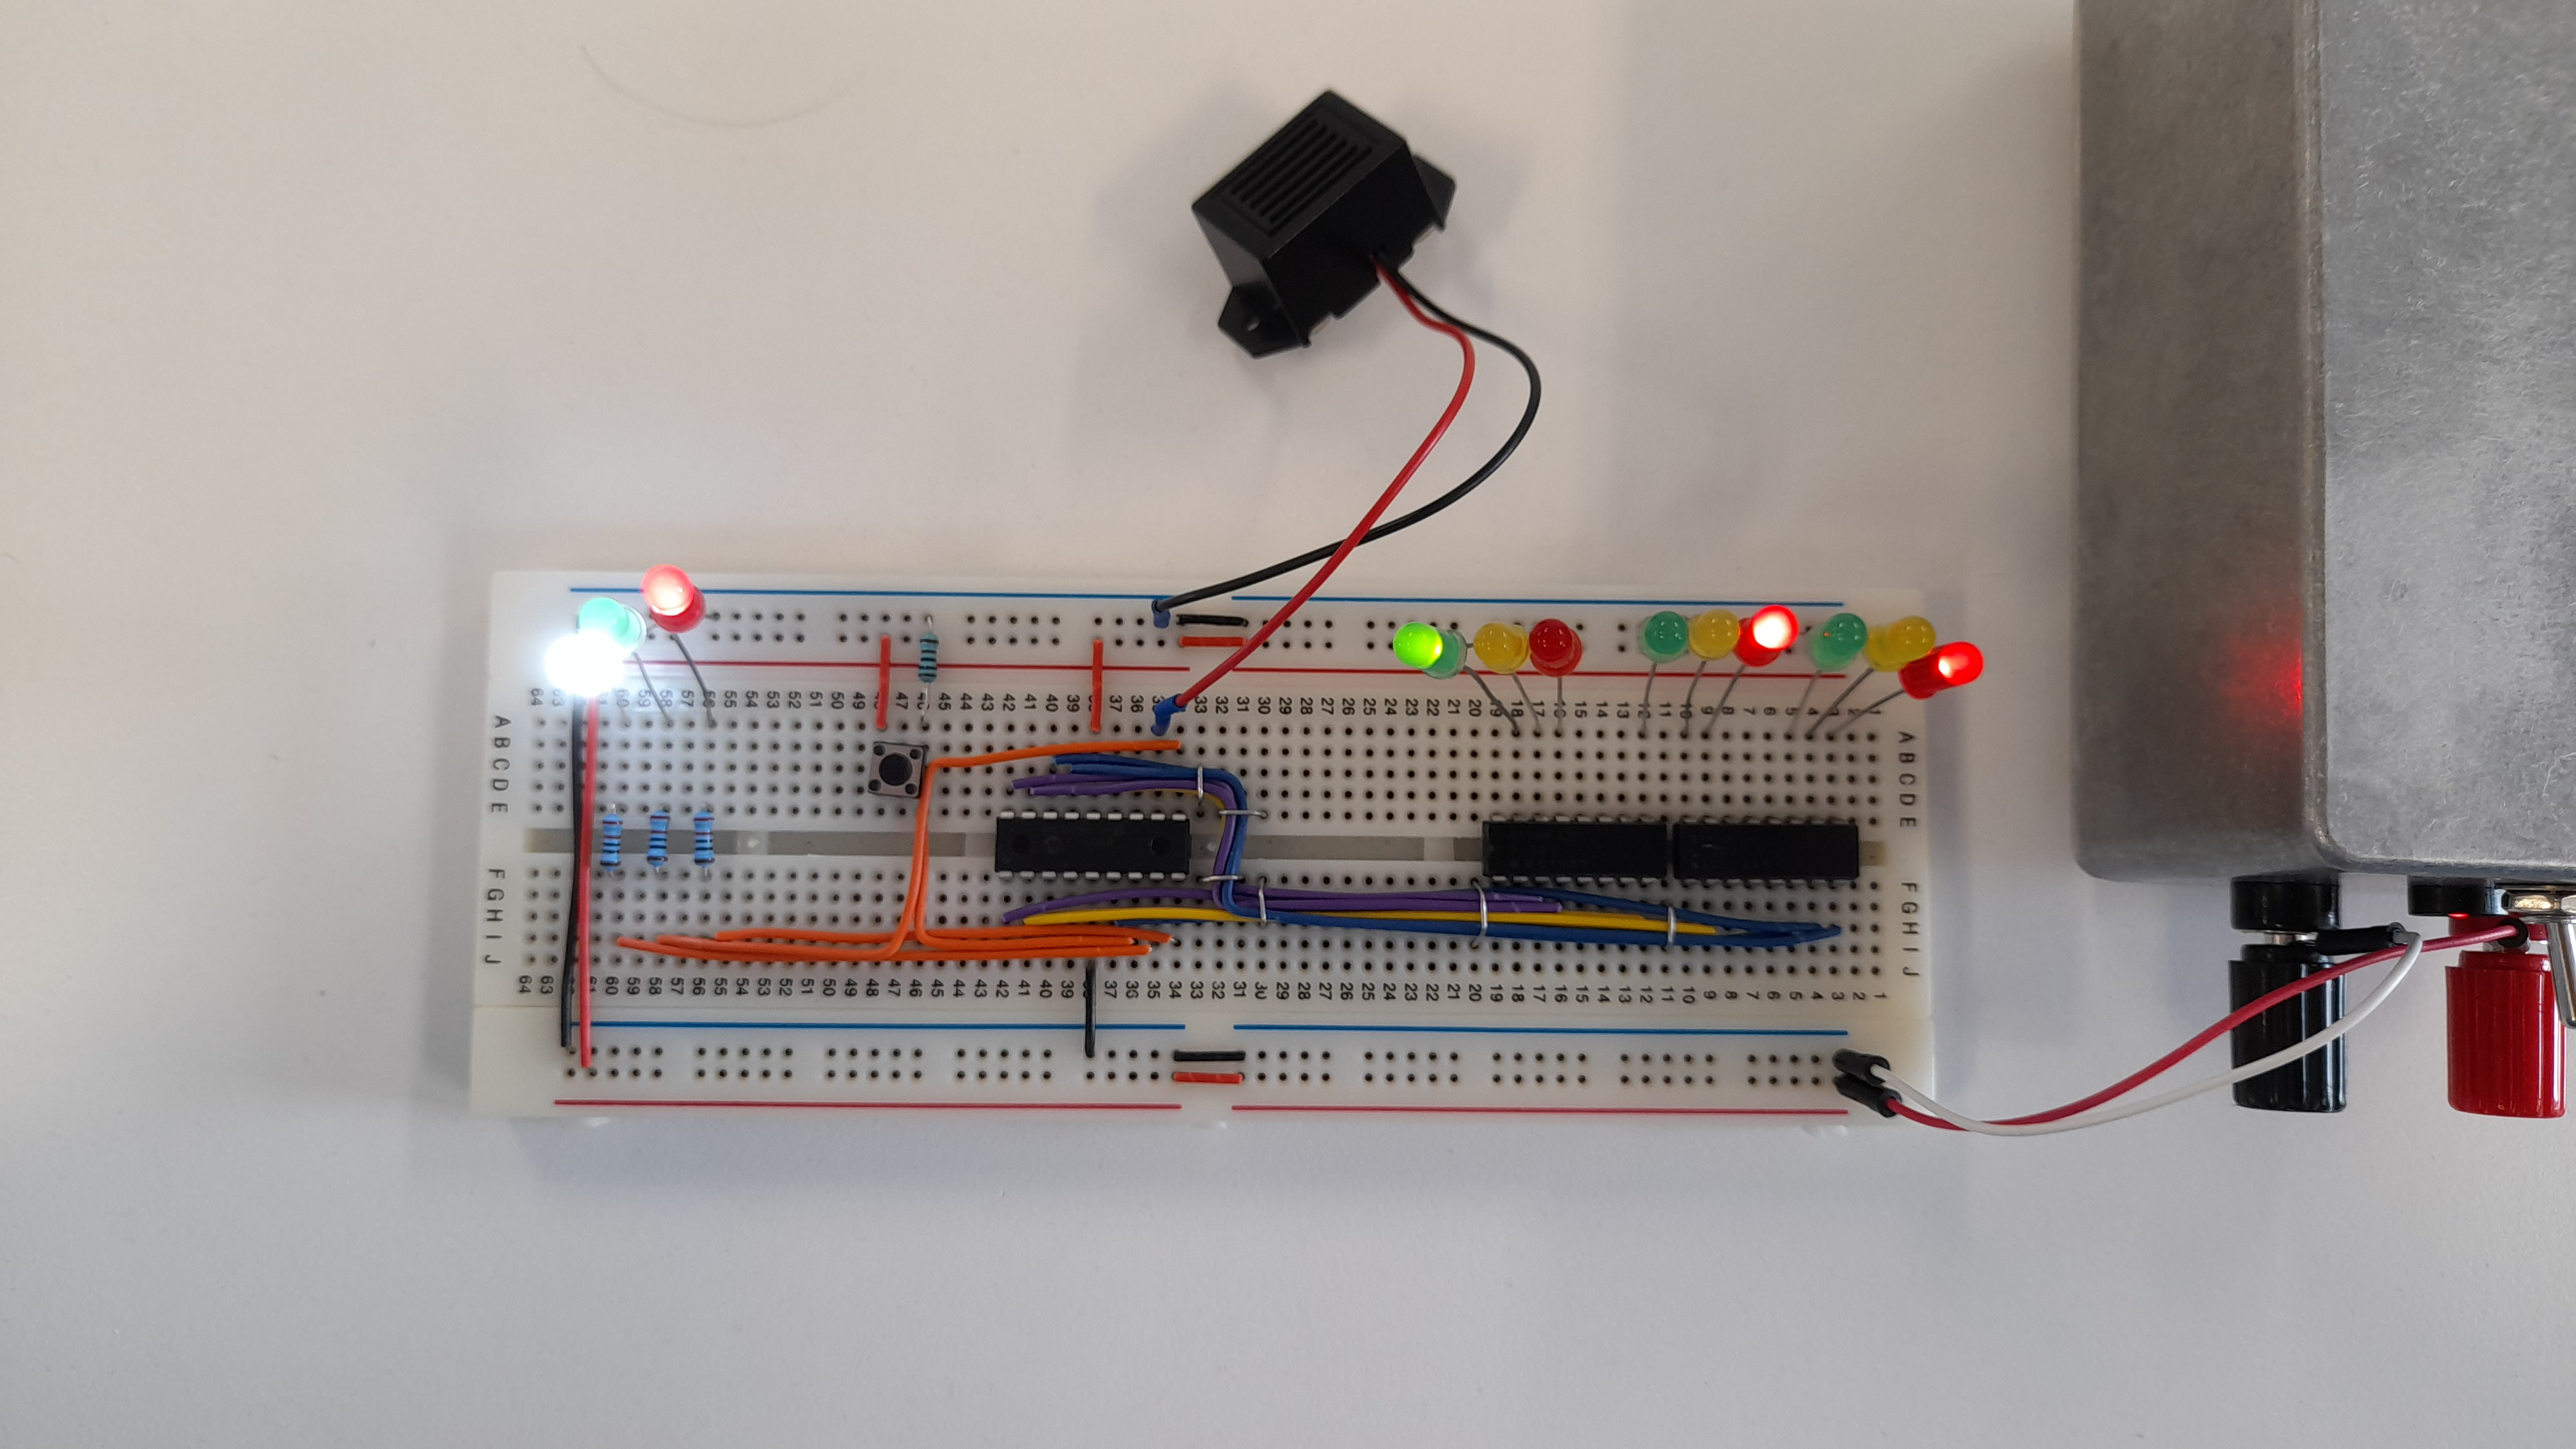
\includegraphics[width=0.9\textwidth]{images/final-testing/state_c_1.jpg}
        \caption{Crossing state 1 - wait button on phase}
        \label{fig:state_c_1}
    \end{minipage}\hfill
    \begin{minipage}{0.45\textwidth}
        \centering
        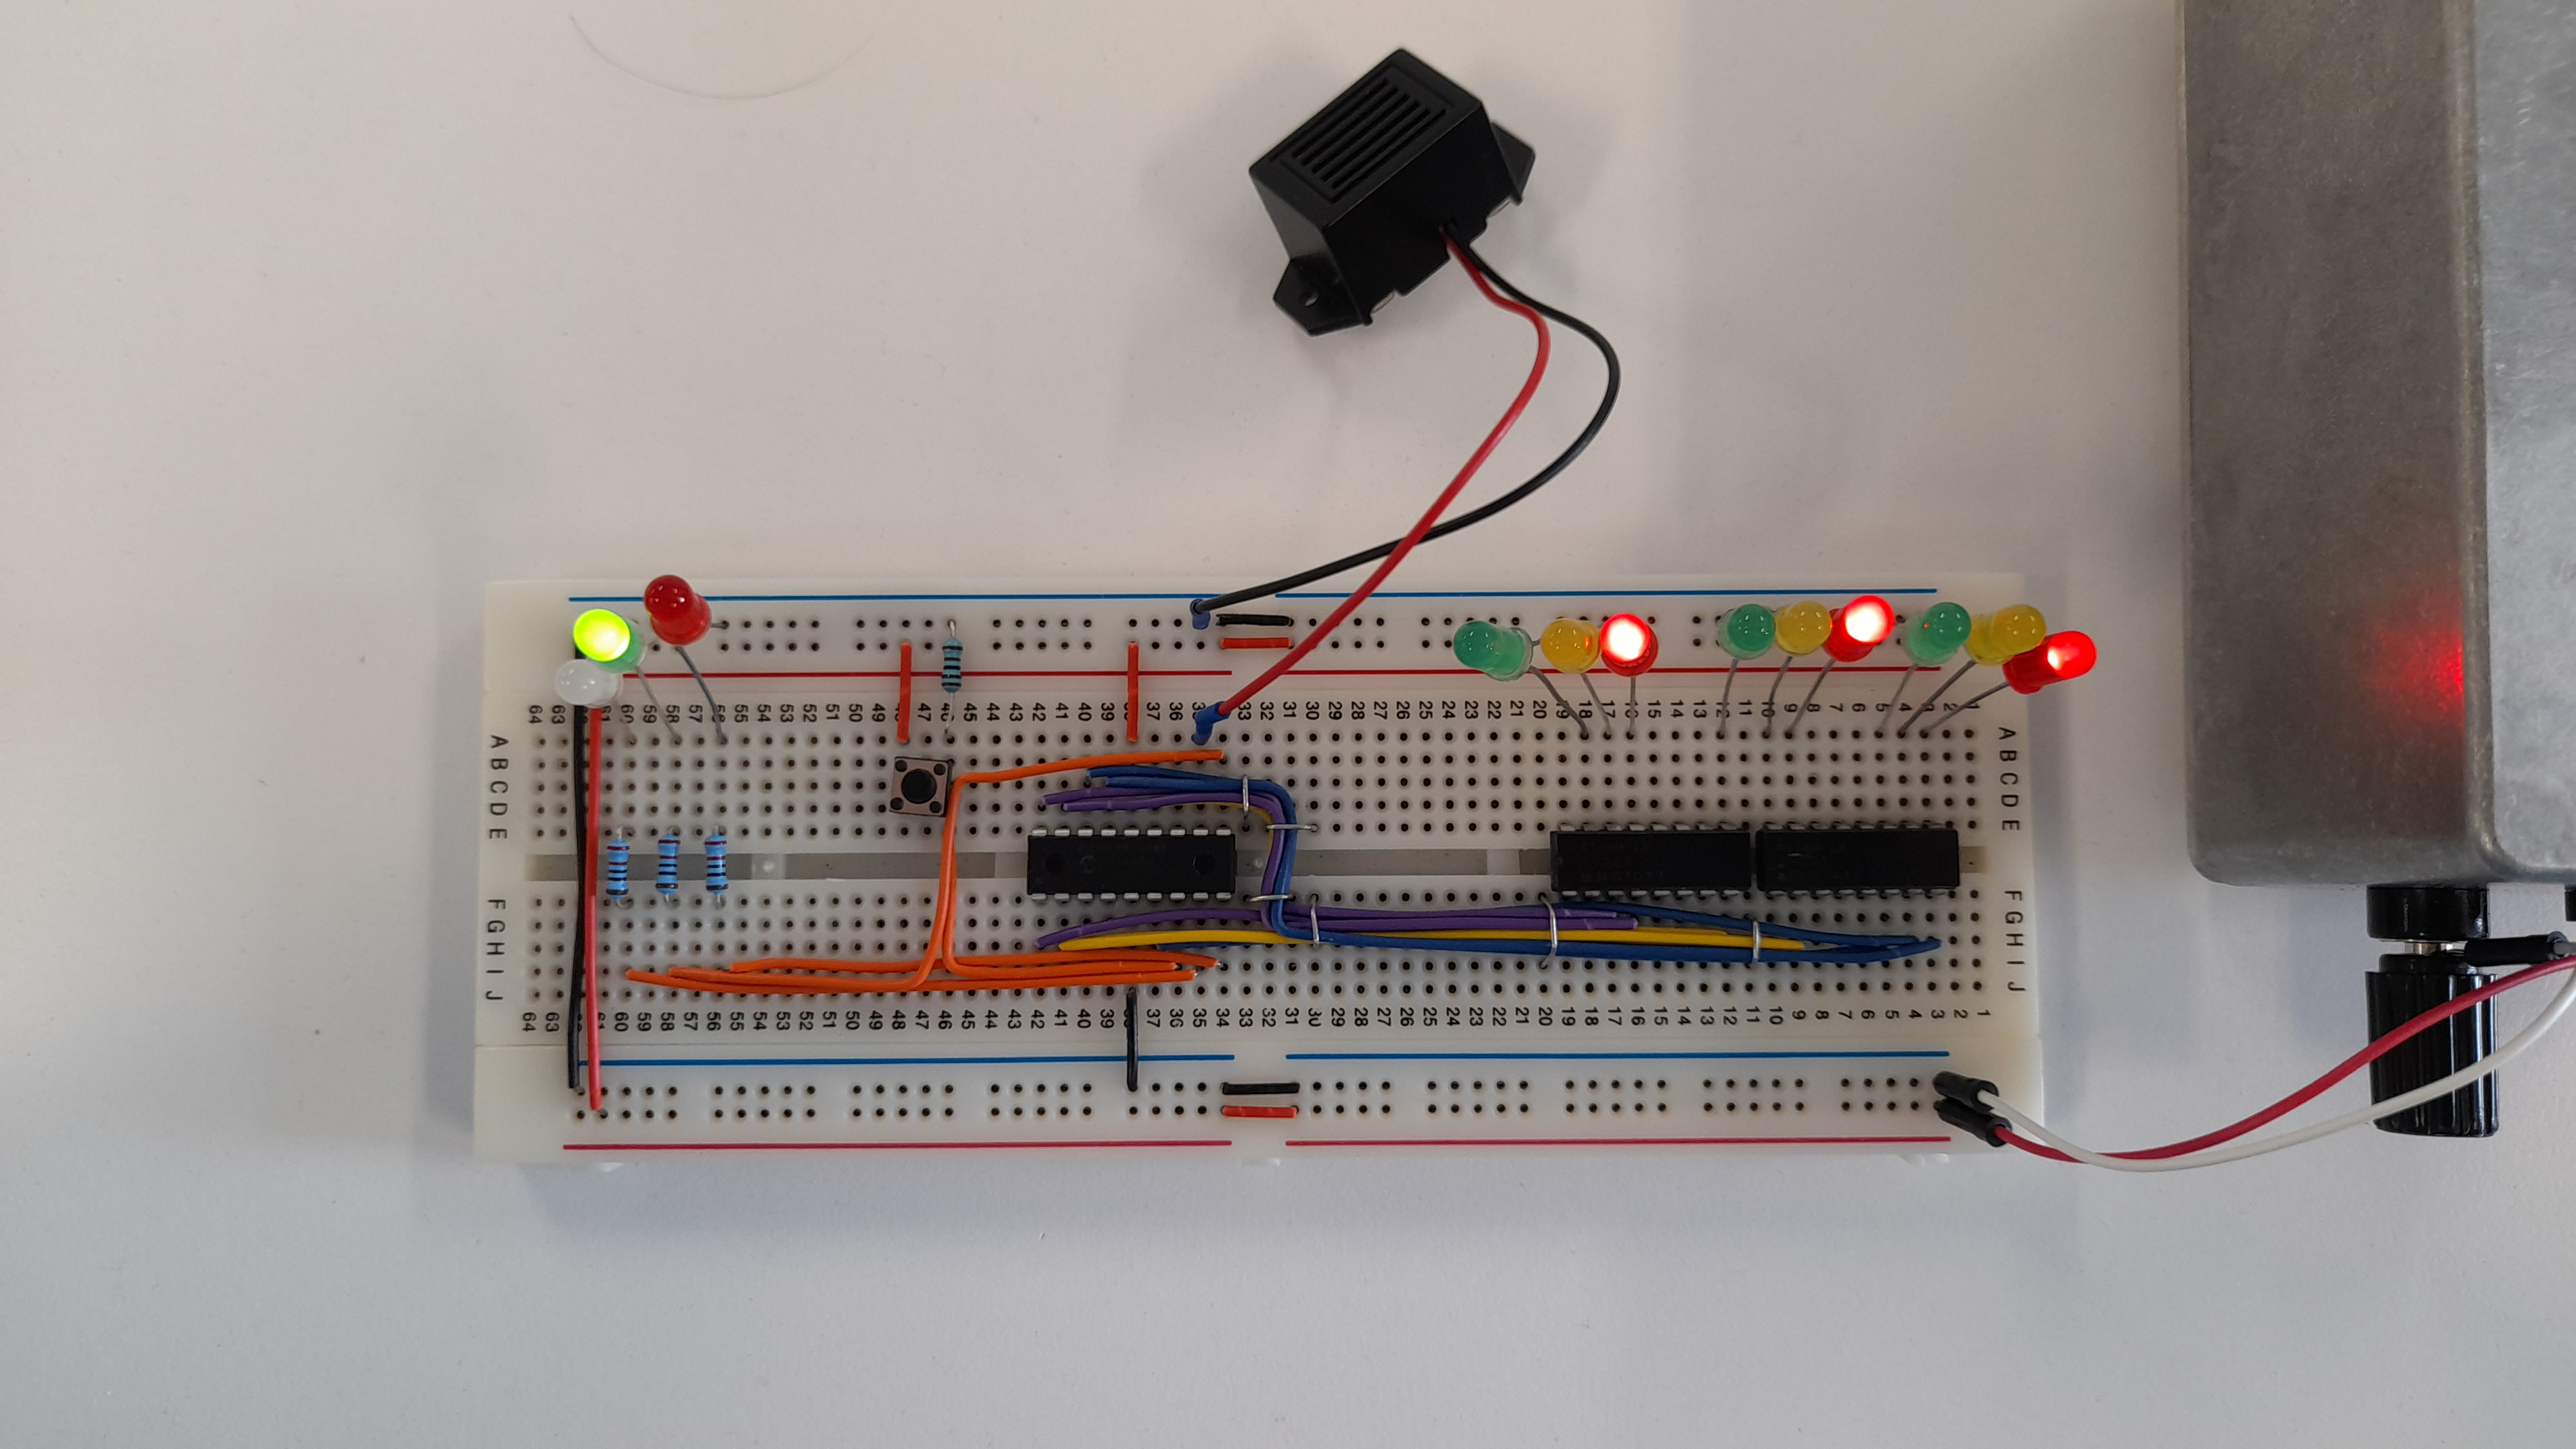
\includegraphics[width=0.9\textwidth]{images/final-testing/state_c_2.jpg}
        \caption{Crossing state 2 - safe to cross phase}
        \label{fig:state_c_2}
    \end{minipage}
\end{figure}
\chapter{Evaluation}
Once I had fully constructed my circuit, I am able to connect it to the power supply and evaluate what I have produced against my success criteria.
\section{Evaluating against Specification}
\begin{itemize}
    \item \textbf{The voltmeter will measure in volts and range from 0V to 5V, in 0.1V increments.}\\ When the voltmeter works, this is achieved. However as the voltmeter doesn't work reliably this point \tempText{red}{cannot be marked as achieved}.
    \item \textbf{The voltmeter will have a sample rate of 1KHz $\pm 400Hz$ times per second. This will be produced by Schmitt Astable with a frequency of 1KHz.}\\ From testing the clock subsystem, I know that the frequency of the clock is $1.36KHz$. This is a suitable deviation from the original success criteria (as it is an increase of less than 400Hz), meaning the clock pulses 1360 times per second. Therefore this point \tempText{Green}{can be marked as achieved}.
    \item \textbf{The voltmeter is accurate to within $\pm0.1V$.}\\ From testing the final circuit, I have found out that when it works, it is accurate within my specified bounds but when it doesn't work it is extremely inaccurate. Therefore this point \tempText{orange}{can be marked as partially achieved}.
    \item \textbf{The voltmeter takes less than 0.5 seconds to adjust its output once a change in voltage is detected.}\\ Despite the fact that the voltmeter was unreliable, I was able to measure the frequency of the clock. This frequency would mean that the clock could complete a full ramp in less than 0.5 seconds. Therefore this point \tempText{Green}{marked as achieved}.
    \item \textbf{The voltmeter should take a +5v, 0V and -5V (within ±0.5V) input.}\\ These are the inputs required for the DAC subsystem, therefore this point \tempText{Green}{can be marked as achieved}.
    \item \textbf{The voltmeter will be easy to use.}\\ From testing and asking the opinions of those who have tested my voltmeter for me, I have found that the voltmeter is easy to use. Therefore this point \tempText{Green}{can be marked as achieved}.
    \item \textbf{The voltage will output to two 7-segment displays; one for the units and one for the tenths.} \\ As seen in my full layout image, there are two 7-segment displays, one of which is used for units and the other for tenths. Therefore this point \tempText{Green}{can be marked as achieved}.
    \item \textbf{The entire circuit will only require human input to connect the analogue voltage.}\\ When the circuit is working, this point is achieved. However as the circuit doesn't work all of the time, this point \tempText{orange}{can be marked as partially complete}.
    \item \textbf{The voltmeter should be as efficient as possible, reducing heat dissipated to the environment.}\\ As my circuit is using a low voltage and current input, there isn't much energy to be dissipated. This low energy input requirement is partially due to the fact that I chose to use CMOS chips rather than TTL. TTL require a much higher operating voltage and current therefore they dissipate a much higher amount of energy. Therefore this point \tempText{Green}{can be marked as achieved}.
\end{itemize}
From evaluating against my specification, I can conclude that this project was not a complete success as only 66\% of the specification points were met. \newline For my project to have been a success, I would have needed an 75\% achievement rate of my success criteria. This would have meant 7 of the points would have to be achieved.

\section{Improvements}
To improve this project, I would troubleshoot further into the cause of the latches not clocking at the right time, then work to fix that issue. Assuming that this is the only issue I come into, then that would allow me to mark the remaining 4 success criteria points as achieved.\newline
A further improvement I could make is to take my layout on breadboards, and use a digital tool to convert it into a PCB. This would reduce the overall physical layout of the circuit as well as reduce the chance for a component to be knocked out. Furthermore, this would improve the noise performance of the circuit and allow for a better grounding arrangement. This would also allow me to implement a better timing system as it would be simpler to construct.

\section{Conclusion}
In conclusion, my system did not meet all of the specification points I put together before constructing it. This means it is not a functioning voltmeter. This was an extremely challenging project however once I understood how the subsystems worked, I was able to design and build them using the knowledge I gained from the theory modules of the course. The most challenging aspect was troubleshooting the many issues I ran into, especially the noise on the output from the DAC.

\appendix
\chapter{Full Code Listing}
\label{app:full-code}

\begin{lstlisting}[language={[x86masm]Assembler}, style=assembly, caption=Full code listing]
;*******************************************************************
;                               TEMPLATE PROVIDED BY CENTRE

;         TITLE:  #### TRAFFIC LIGHTS CONTROL SYSTEM #####
;         AUTHOR: ######## THOMAS BOXALL #########
;         DATE:   ####### 17-03-2022 ######
;

;******************************************************************
; PROGRAM DESCRIPTION:
;
; ####  State here what the program does  #######
;
;*********************************************************************
;			DEFINITIONS
;*********************************************************************
    list    p=16F88             	; tells the assembler which PIC chip to program for
    radix	dec                 	; set default number radix to decimal
    ;radix	hex                 	uncomment this to  set  radix to hex
    __config h'2007', 0x3F50	; internal oscillator, RA5 as i/o, wdt off
    __config h'2008', 0x3FFF	
    errorlevel -302             	; hide page warnings

W           	EQU h'00'	; pointer to Working register
F            	EQU h'01'	; pointer to file

;****** REGISTER USAGE ******

;For PIC16F88, user RAM starts at h'20'. The following definitions
;will be found useful in many programs.

; Register page 1
TRISA	EQU h'85'	; data direction registers
TRISB	EQU h'86'
OSCCON	EQU h'8F'	; internal oscillator speed
ANSEL	EQU h'9B'	; ADC port enable bits

; Register page 0        
STATUS	EQU h'03' 	; status
PORTA	EQU h'05'	; input / output ports
PORTB	EQU h'06'
INTCON	EQU h'0B'	; interrupt control
ADRESH	EQU h'1E'	; ADC result
ADCON0	EQU h'1F'	; ADC control

B0	EQU h'20'	; general use byte registers B0 to B27
B1	EQU h'21'
B2	EQU h'22'
B3	EQU h'23'
B4	EQU h'24'
B5	EQU h'25'
B6	EQU h'26'
B7	EQU h'27'
B8	EQU h'28'
B9	EQU h'29'
B10	EQU h'2A'
B11	EQU h'2B'
B12	EQU h'2C'
B13	EQU h'2D'
B14	EQU h'2E'
B15	EQU h'2F'
B16	EQU h'30'
B17	EQU h'31'
B18	EQU h'32'
B19	EQU h'33'
B20	EQU h'34'	; used in interrupt routine
B21	EQU h'35'	; used in interrupt routine
B22	EQU h'36'
B23	EQU h'37'
B24	EQU h'38'
B25	EQU h'39'
B26	EQU h'3A'
B27	EQU h'3B'

WAIT1	EQU h'3C'	; counters used in wait delays
WAIT10	EQU h'3D'
WAIT100	EQU h'3E'
WAIT1000	EQU h'3F'
ADCTEMP	EQU h'40'	; adc loop counter

;my vars below
loopX EQU h'41' ;loop counter variable x
loopY EQU h'42' ;loop counter variable y

;****** REGISTER BITS ******

C          	EQU h'00' 	; carry flag
Z           	EQU h'02'	; zero flag
RP0         	EQU h'05'	; register page bit
INT0IF      	EQU h'01'	; interrupt 0 flag
INT0IE     	EQU h'04'	; interrupt 0 enable
GIE         	EQU h'07'	; global interrupt enable

;*********************************************************************
;			VECTORS
;*********************************************************************

;The PIC16F88 reset vectors 

    ORG     h'00'       	; reset vector address
	goto 	start  	; goes to first instruction on reset/power-up
    ORG     h'04'     	; interrupt vector address
	goto	interrupt
;
;*********************************************************************
;			SUBROUTINES
;*********************************************************************
; Predefined wait subroutines - wait1ms, wait10ms, wait100ms, wait1000ms

wait1ms		; (199 x 5) + 5 instructions = 1000us = 1ms @ 4MHz resonator
	movlw d'199'    ; 1
	movwf WAIT1  	; 1
loop5ns
	clrwdt         	; 1 this loop 1+1+1+2 = 5 instructions
	nop            	; 1
	decfsz WAIT1,F	; 1 
	goto loop5ns	; 2
	nop            	; 1
	return          	; 2
wait10ms
	movlw d'10'     	; 10 x 1ms = 10ms
	movwf WAIT10	
loop10ms
	call 	wait1ms	
	decfsz 	WAIT10,F	
	goto 	loop10ms	 
	return          

wait100ms
	movlw d'100'	; 100 x 1ms = 100ms
	movwf WAIT100	
loop100ms
	call 	wait1ms	
	decfsz 	WAIT100,F
	goto 	loop100ms	 
	return          

wait1000ms
	movlw 	d'10'     ; 10 x 100ms = 1000ms
	movwf 	WAIT1000	 
loop1000ms
	call 	wait100ms	
	decfsz 	WAIT1000,F
	goto 	loop1000ms	
	return          

; MY SUBROUTINES BELOW

;wait five seconds and check the pedestian crossing while looping
;wait5SecondsButtonCheck
;	;setup times etc for loops
;	movlw d'50' ;set val of 50 into working register
;	movf loopX ;move 50 into loopX
;	movlw d'100' ;set val of 100 into working regsiter
;	movf loopY ;move 100 into loopY
;	
;	movf loopY, 0  ; move loopY into W register
;	sublw d'100' ;subtract W register (loopY) from 100
;	btfss STATUS, Z ;skip next line if the zero bit is set (finished the loop)
;	goto contY ;goto the continue working on loopY


;contY	movf loopY, 0 ;moove loopY into W register
	

waitFiveSecondsCheckButton
	;first, stary loop x
	movlw d'5' ;set val of 5 into w register
	;movf loopX ; move the val in the working register (5) into loopX

topX decfsz loopX, 1 ;decrement loopX and place the new value back into loopX
	goto startY ;line skipped if result is 0
	return ;if result of loopX - 1 is 0, run this line

startY movlw d'101'; ;set value of 101 into w register
	;movf loopY ;move value in working register (101) into loopY

topY decfsz loopY, 1 ;decrement loopY and place new value back into loopY
	goto finalPart ;goto final part of the function
	goto topX ;run if loopY = 0

finalPart call checkButton
	call wait10ms ;wait for 10ms function
	goto topY ;go back up to topY and loop around again
;end of function


waitOneSecondCheckButton
	movlw d'101' ;set value of 101 into w register
	movf loopY ;move val from working register into loopY
topZ decfsz loopY, 1 ;decrement loopY and place new value back into loopY
	goto finalPart2 ;goto final part of the function (if loopyY>0)
	return ; go back to where called from if loopY=0
finalPart2 call checkButton
	call wait10ms ;wait for 10ms function
	goto topZ ;go back up to the decrement of loopY
; end of function


;function to check the button
checkButton
	btfss PORTB, 1 ;skip next line of code if button pressed (active high)
	return ;can go back to where called from
	bsf PORTB, 2 ;turn white wait LED on
	return ;go back to main code
;end of function


; function to cycle the pedestrian crossing
cycleCrossing
	bcf PORTB, 2 ;turn off red wait LED
	bcf PORTB, 3 ;turn off red stop LED
	bsf PORTB, 4 ;turn on green go LED
	bsf PORTB, 5 ;turn on buzzer
	call wait1000ms ;wait 1second
	call wait1000ms ;wait 1second
	call wait1000ms ;wait 1second
	;now have waited 3seconds so invert things and return to main sequence
	bcf PORTB, 4 ;turn off green go LED
	bsf PORTB, 3 ;turn on red stop LED
	bcf PORTB, 5 ;turn off buzzer
	return ;return to the main program
;end of function

greenTrafficLightSequence
	bsf PORTA, 4 ;turn on amber led
	call waitOneSecondCheckButton ;wait 5s
	call waitOneSecondCheckButton
	call waitOneSecondCheckButton
	call waitOneSecondCheckButton
	call waitOneSecondCheckButton
	bcf PORTA, 4 ;turn off amber led
	bcf PORTA, 3 ;turn off red led
	bsf PORTB, 7 ;turn on greeen led
	call waitOneSecondCheckButton ;wait 10s
	call waitOneSecondCheckButton
	call waitOneSecondCheckButton
	call waitOneSecondCheckButton
	call waitOneSecondCheckButton
	call waitOneSecondCheckButton 
	call waitOneSecondCheckButton
	call waitOneSecondCheckButton
	call waitOneSecondCheckButton
	call waitOneSecondCheckButton
	bcf PORTB, 7 ;turn off green led
	bsf PORTA, 4 ;turn on amber led
	call waitOneSecondCheckButton ;wait 5s
	call waitOneSecondCheckButton
	call waitOneSecondCheckButton
	call waitOneSecondCheckButton
	call waitOneSecondCheckButton
	bsf PORTA, 3 ;turn on red led
	bcf PORTA, 4 ;turn off amber led
	return ;go back to main code
;end of function

pinkTrafficLightSequence
	bsf PORTA, 1 ;turn on amber led
	call waitOneSecondCheckButton ;wait 5s
	call waitOneSecondCheckButton
	call waitOneSecondCheckButton
	call waitOneSecondCheckButton
	call waitOneSecondCheckButton
	bcf PORTA, 1 ;turn off amber led
	bcf PORTA, 0 ;turn off red led
	bsf PORTA, 2 ; turn on greeen led
	call waitOneSecondCheckButton ;wait 10s
	call waitOneSecondCheckButton
	call waitOneSecondCheckButton
	call waitOneSecondCheckButton
	call waitOneSecondCheckButton
	call waitOneSecondCheckButton 
	call waitOneSecondCheckButton
	call waitOneSecondCheckButton
	call waitOneSecondCheckButton
	call waitOneSecondCheckButton
	bcf PORTA, 2 ;turn off green led
	bsf PORTA, 1 ;turn on amber led
	call waitOneSecondCheckButton ;wait 5s
	call waitOneSecondCheckButton
	call waitOneSecondCheckButton
	call waitOneSecondCheckButton
	call waitOneSecondCheckButton
	bsf PORTA, 0 ;turn on red led
	bcf PORTA, 1 ;turn off amber led
	return ;go back to main code
;end of function

blueTrafficLightSequence
	bsf PORTA, 7 ;turn on amber led
	call waitOneSecondCheckButton ;wait 5s
	call waitOneSecondCheckButton
	call waitOneSecondCheckButton
	call waitOneSecondCheckButton
	call waitOneSecondCheckButton
	bcf PORTA, 7 ;turn off amber led
	bcf PORTA, 6 ;turn off red led
	bsf PORTB, 0 ; turn on greeen led
	call waitOneSecondCheckButton ;wait 10s
	call waitOneSecondCheckButton
	call waitOneSecondCheckButton
	call waitOneSecondCheckButton
	call waitOneSecondCheckButton
	call waitOneSecondCheckButton 
	call waitOneSecondCheckButton
	call waitOneSecondCheckButton
	call waitOneSecondCheckButton
	call waitOneSecondCheckButton
	bcf PORTB, 0 ;turn off green led
	bsf PORTA, 7 ;turn on amber led
	call waitOneSecondCheckButton ;wait 5s
	call waitOneSecondCheckButton
	call waitOneSecondCheckButton
	call waitOneSecondCheckButton
	call waitOneSecondCheckButton
	bsf PORTA, 6 ;turn on red led
	bcf PORTA, 7 ;turn off amber led
	return ;go back to main code
;end of function

checkPedestrian
	;function to check if the wait led is on
		;if yes - cycle pedestrian crossing
		;if no - return to main 
	btfsc PORTB, 2 ;skip next line if wait led NOT on therefore if on, run next line
	call cycleCrossing
	return
;end function

; Predefined ADC subroutines - readadc0, readac1, readadc2

readadc0
	movlw	b'00000001'	; setup mask for pin A.0
	call	readadc	; do the adc conversion
	movwf	B0         	; save result in B0
	return
readadc1
	movlw	b'00000010'	; setup mask for pin A.1
	call	readadc	; do the adc conversion
	movwf	B1          	; save result in B1
	return
readadc2
	movlw	b'00000100' 	; setup mask for pin A.2
	call	readadc	; do the adc conversion
	movwf	B2          	; save result in B2
	return

readadc
; Generic sub routine to read ADC 0, 1 or 2 (pass appropriate mask in W)
; To start conversion we need mask (001, 010, 100) in ANSEL bits 0-2
; but the actual channel number (0, 1, 2) in ADCON0 channel select bits
; Then set the ADCON0, GO bit to start the conversion

	bsf     	STATUS,RP0	; select register page 1
	movwf	ANSEL		; move mask value 001,010,100 into ANSEL
	bcf     	STATUS,RP0	; select register page 0
	movwf	ADCTEMP	; 00000??? 	get mask value
	rlf     	ADCTEMP,F	; 0000???x	rotate twice
	rlf     	ADCTEMP,W	; 000???xx
	andlw	b'00011000'	; 000??000	mask off the unwanted bits
	iorlw	b'00000001'	; 000??001	set the 'ADC on' bit	 
	movwf	ADCON0	; move working into ADCON0
    	movlw   	d'10'      	; 10 x 3 = 30us acquistion time
    	movwf   ADCTEMP    	; re-use ADC1 register as a counter
loopacq
    	decfsz  	ADCTEMP,F  	; loop around to create short delay
    	goto    	loopacq    	; each loop is 1+2 = 3 instructions = 3us @ 4MHz
	bsf     	ADCON0,2	; now start the conversion
loopadc
	clrwdt      		; pat the watchdog
	btfsc	ADCON0,2	; is conversion finished?
	goto	loopadc	; no, so wait a bit more
	movf	ADRESH,W	; move result into W
	return          		; return with result in W

; NOTE for PICAXE users:  the following four specific subroutines and two instructions are not supported by PICAXE compiler
readtemp1:
readtemp2:
readtemp3:
debug:
lcd:
	clrw               		; instruction not supported by this template
	return			; instruction not supported by this template
;*********************************************************************
;			MAIN PROGRAM
;*********************************************************************

;****** INITIALISATION ******
start
	bsf     	STATUS,RP0	; select register page 1
	movlw  	b'01100000'	; set to 4MHz internal operation
	movwf	OSCCON	
	clrf	ANSEL		; disable ADC (enabled at power-up)
	bcf     	STATUS,RP0	; select register page 0

;The data direction registers TRISA and TRISB live in the special register set. A '1' in
;these registers sets the corresponding port line to an Input, and a
;'0' makes the corresponding line an output.

Init
	clrf    	PORTA     	; make sure PORTA output latches are low
    	clrf    	PORTB     	; make sure PORTB output latches are low   
	bsf     	STATUS,RP0	; select register page 1
;Modify the next line to correspond with your input output reqirements	
	movlw	b'00000000'	; set port A data direction (0 = output bit, 1 = input bit)
	movwf	TRISA		; 
;Modify the next line to correspond with your input output requirements	
	movlw	b'00000010'	; set port B data direction (0 = output bit, 1 = input bit)
	movwf	TRISB		; 	
	bcf     	STATUS,RP0	; select register page 0

;****** MAIN PROGRAM ******
;************* remove semicolons from next two lines to enable interrupt routine************
   	; bsf    	INTCON,INT0IE  ; set external interrupt enable
   	; bsf    	INTCON,GIE        ; enable all interrupts 

main 
;*********************************************************************

; YOUR PROGRAM GOES HERE ######################

	;first turn on all stop leds
	bsf PORTA, 0 ;turn on pink set stop eld
	bsf PORTA, 3 ;turn on green set stop led
	bsf PORTA, 6 ;turn on blue set stop led
	bsf PORTB, 3 ;turn on pedestrian stop led

mTop call pinkTrafficLightSequence
	call checkPedestrian
	call greenTrafficLightSequence
	call checkPedestrian
	call blueTrafficLightSequence
	call checkPedestrian
	goto mTop

;*********************************************************************
;			INTERRUPT SERVICE ROUTINE
;*********************************************************************

W_SAVE	EQU B20     		; backup registers used in interrupts

interrupt
	movwf 	W_SAVE 	; Copy W to save register
	
    	btfss  	INTCON,INT0IF  ; check correct interrupt has occurred
    	retfie                		; no, so return and re-enable GIE

;**********The interrupt service routine (if required) goes here*********

   	bcf    INTCON,INT0IF  	; clear interrupt flag 
	movf   W_SAVE,W       	; restore W
	retfie             		; return and re-set GIE bit
	
    	END                		; all programs must end with this

 
\end{lstlisting}
\chapter{Full Schematic}
\label{chap:schematic}
\begingroup
\let\clearpage\relax

\begin{figure}[H]
    \centering
    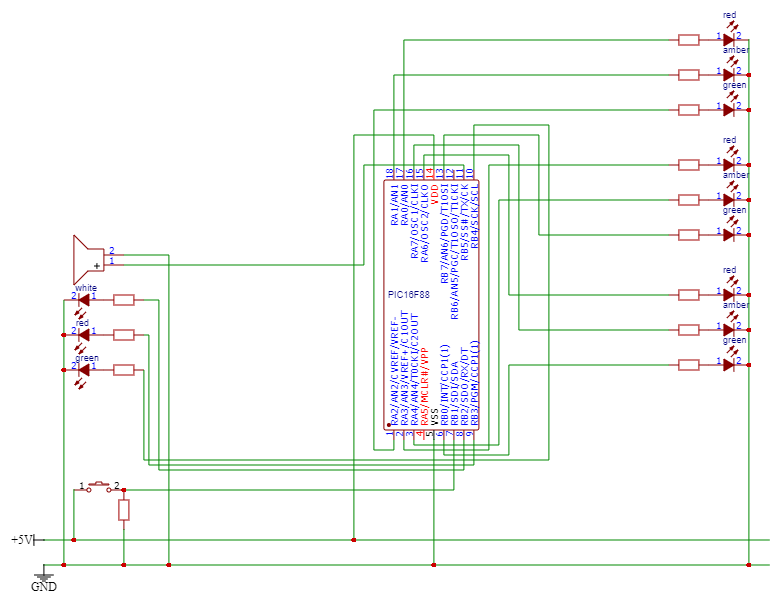
\includegraphics[width=0.9\textwidth]{images/Schematic_A-level-microcontroller_2022-03-20.png}
    \caption{Schematic of the circuit}
    \label{fig:fullSchematic}
\end{figure}
\endgroup

\chapter{Final Physical Layout}
\label{chap:finalLayout}

\begin{figure}[H]
    \centering
    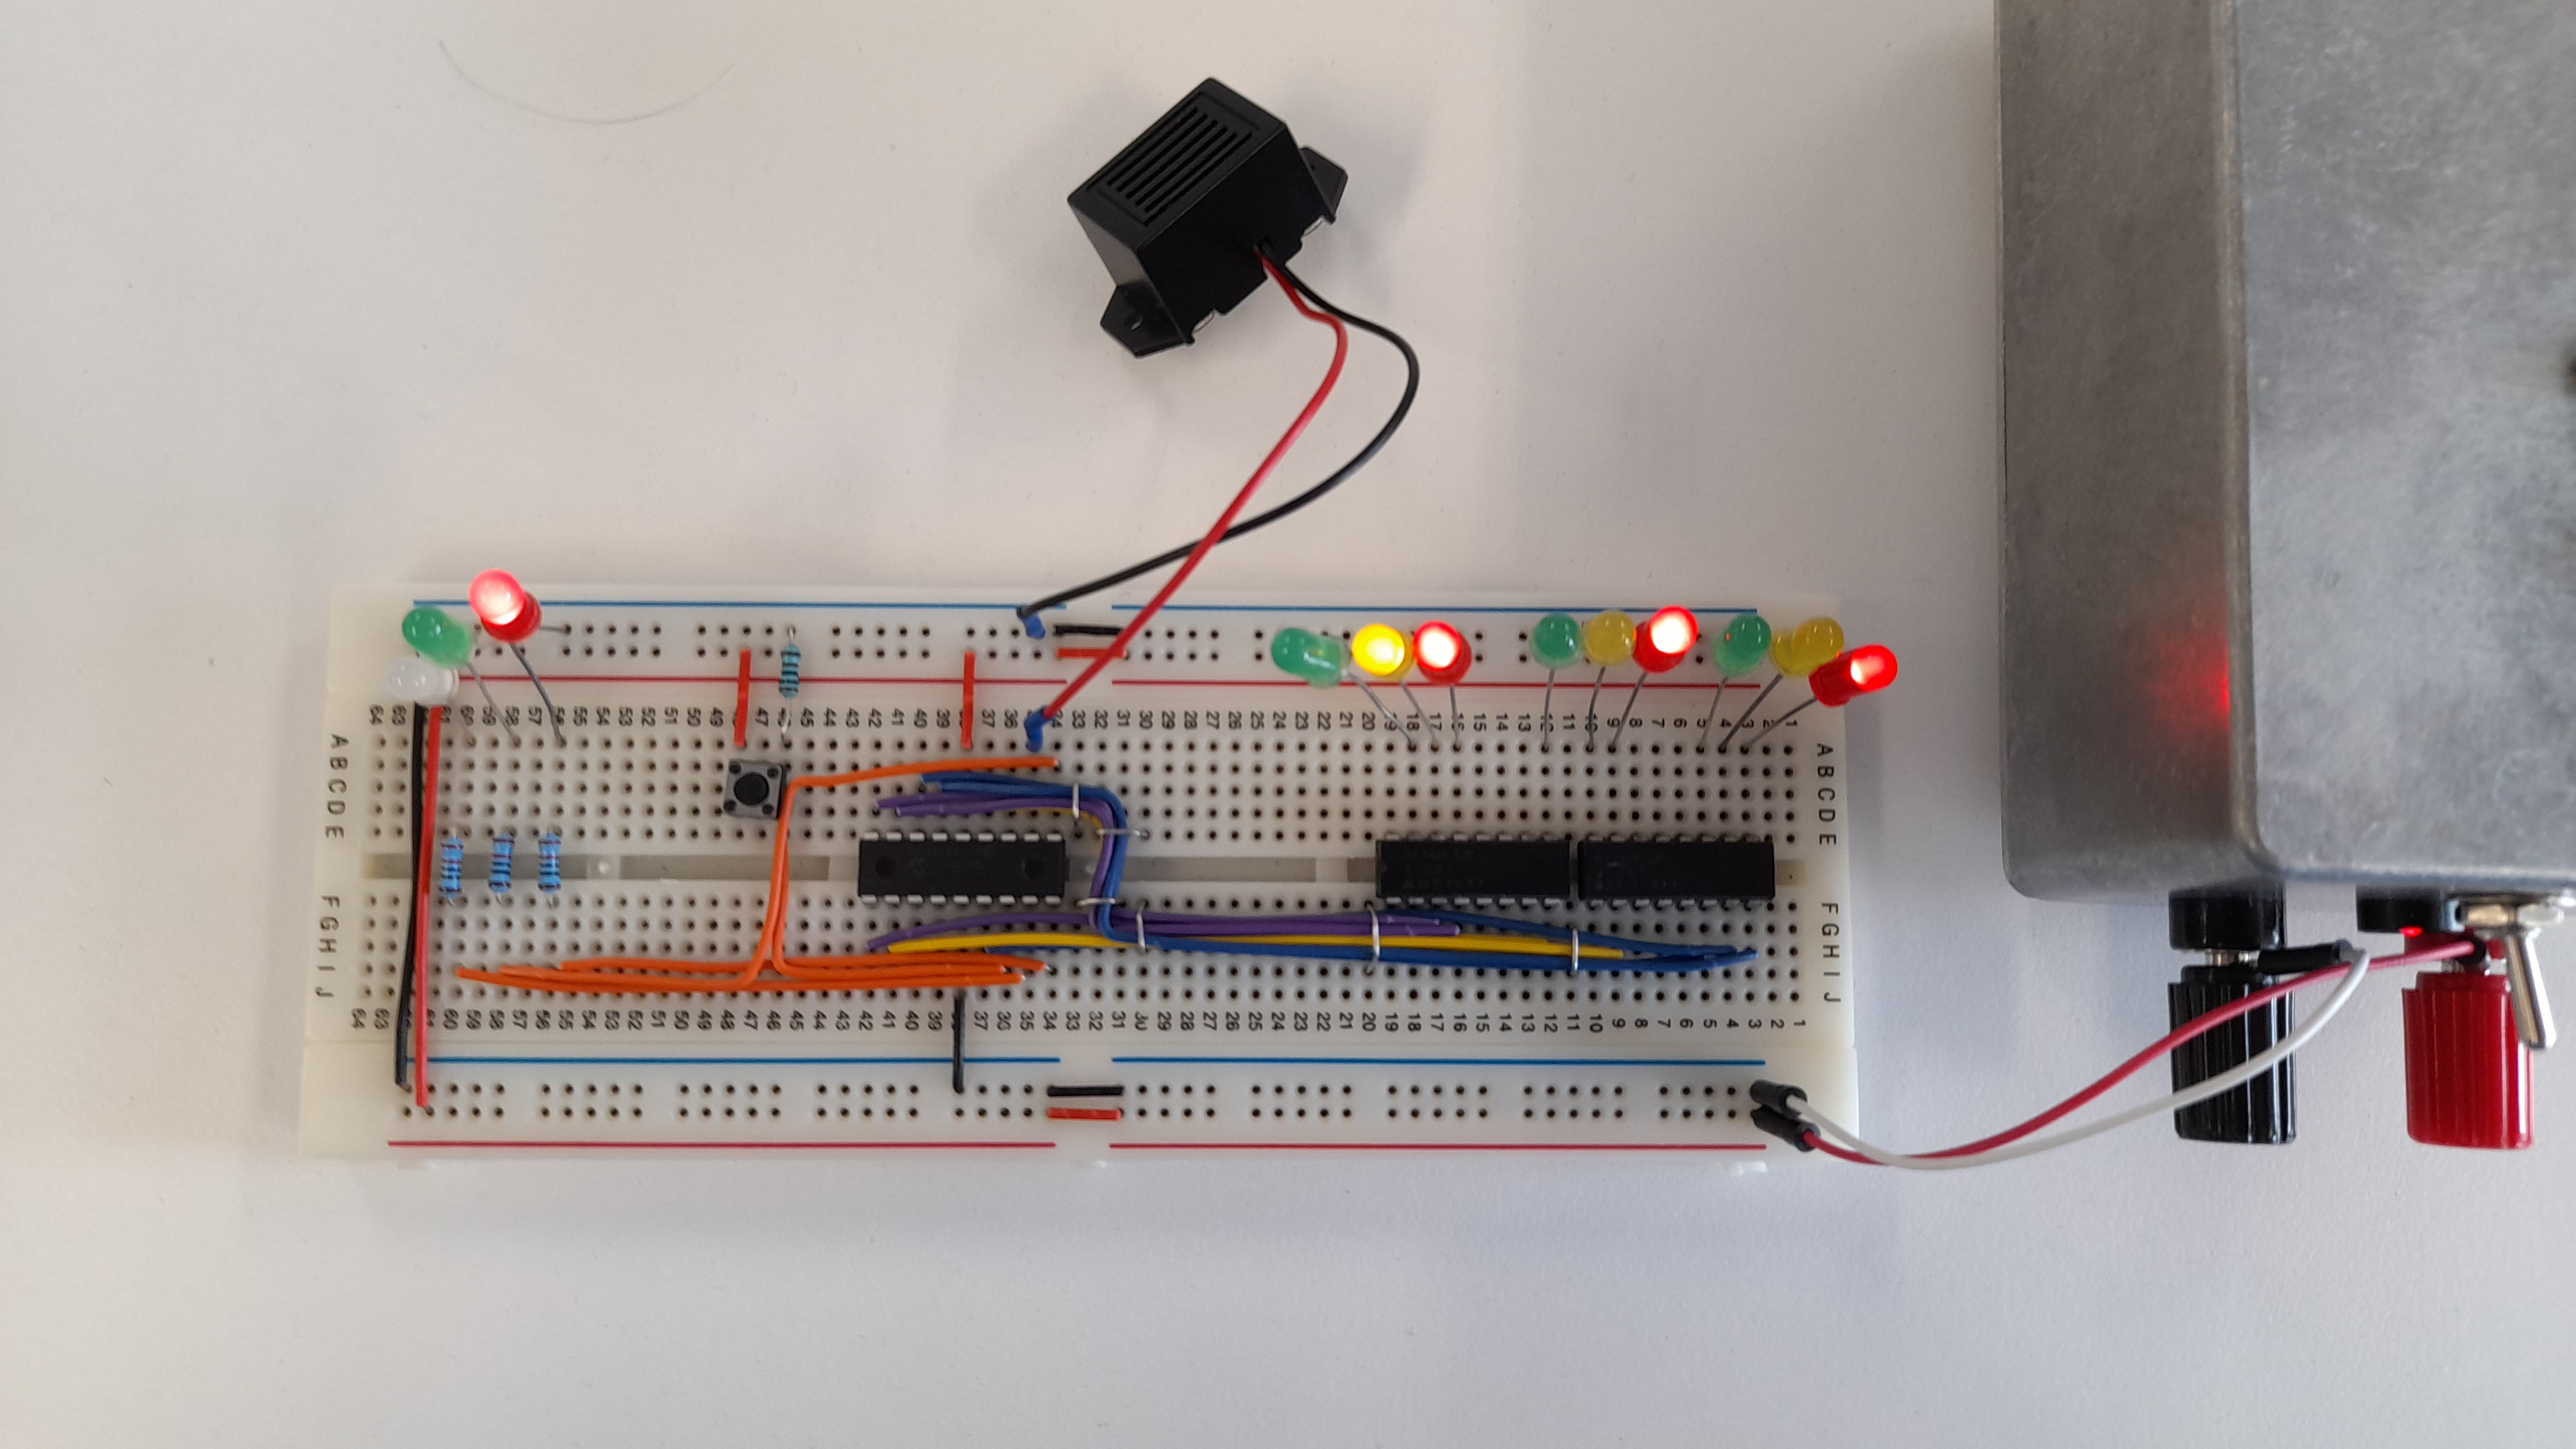
\includegraphics[width=0.9\textwidth]{images/final-testing/state_1.jpg}
    \caption{Final physical layout}
    \label{fig:finalPhysicalLayout}
\end{figure}


\end{document}
